%TODO: Revise method section
%TODO: Create formulation section
%TODO: Create results section

%TODO:
%	Formulation Section
%	Figures
%		Main diagram - break it up into pieces with just text
%		UVL three-axis diagram
%		Replace C with (pi,s)
%	Method:
%		Unprojection Consistency Loss
%		Texture Reality Loss

%TODO:
%	Formulation Section
%	Figures: Main diagram - break it up into pieces with just text
%	Figures: UVL three-axis diagram
%	Method:	Unprojection Consistency Loss
%	Method:	Texture Reality Loss


%ALL CURRENTLY USED TERMS:

%RULES:
%    - Lower case: Belongs to an upper case thing

%     L - num labels
%     N - batch size
%     T - translator
%     A, B - domains
%     Tba
%     Tab
%     tau - texture       !!!!! MUST CHANGE
%			TO DO: replace it with psi ψ, the triton symbol!
%     pi - projection
%     p - photo
%     s - scene
%     l_TR
%     l_UC
%     l_ADV
%     l_REC
%     l_CYC
%     l_T
%     i - texture index
%     f_i - fourier frequency
%     M - MLP for texture network
%     u,v,l,r,g,b - channel values
%     u - unprojections  !!!!!! MUST CHANGE
%          make it capitalized. Unprojection should be denoted by U - it's too intuitive not to.
%     sigma - standard deviation
%     mu - mean
%     E_A, E_B
%     D_A, D_B
%     G_A, G_B

%     similarity(x,y) = MSSSIM(L2(x,y)


% FIXING NOTATION WILL BE HARD :(
% GO OVER WITH XIANG AND JINGHUAN TOMORROW
%     In this paper I use 1-based indexing to make notation simpler.
%
%     s, pi in N,3,H,W - height width
%              i,c,x,y
%     All values between 0 and 1
%
%     I: {1/L, 2/L, ... L/L} -> {1, 2, ... L}  ;   I(l) = l*L
%          I is a discrete mapping from continous label values l to discrete texture indices.
%          It can be nonlinear, as long as its consistent.
%     
%     ψ_i: R2 -> R3   for   i \in {1,2 ... L}
%
%     pi_{n,c,x,y} = ψ_  {I(s_{n,1,x,y})}  (s_{n,2,x,y},s_{n,3,x,y})
%
%     EXPLAINING L_UC IS WAY TO BURDENSOME. We have to talk about weighted standard deviations of unprojections that have a separate unprojection resolution (128x128) etc.
%	  l_UC = total mean across all dims of sigma
%     sigma \in R^{L x C x 128 x 128} is the standard deviation of u in the channel dimension, weighted...
%     !!! I shouldn't have to do this; the other paper didn't!!!
%     u.sum_{N,C,u,v}
%



\newcommand{\msssim}{\text{msssim}}


\newcommand{\Tab}{T_{A\rightarrow B}}
\newcommand{\Tba}{T_{B\rightarrow A}}
\newcommand{\pih}{\hat{\pi}}
\newcommand{\sh}{\hat{s}}
\newcommand{\ph}{\hat{p}}
\newcommand{\pis}{\pi,s} % pi and s pairs from domain A
\newcommand{\pish}{\pih,\sh} % pi and s pairs from domain A
\newcommand{\ppis}{(\pis)} %Parenthesized pis
\newcommand{\ppish}{(\pish)} %Parenthesized pis

\newcommand{\toN}{^{1\dots N}}
% \newcommand{\toNL}{_{1\dots B,\text{ } 1\dots L}}
\newcommand{\toNL}{^{1\dots N, 1\dots L}}
\newcommand{\toL}{^{1\dots L}}

\newcommand{\lUC}{\ell_{UC}}
\newcommand{\lTR}{\ell_{TR}}
\newcommand{\eqand}{\ \ \ \text{ and }\ \ \ }
\newcommand{\eqwhere}{\ \ \ \text{ where }\ \ \ }
\newcommand{\real}{\mathbb{R}}

% \newcommand{\similar}{\text{similarity}}
\newcommand{\similar}{\Omega}
\newcommand{\unprojection}{\omega}
\newcommand{\expectation}{\mathop{\mathbb{E}}}
\newcommand{\lsum}{\sum\limits}


%%%%%%%%%%%%BIG TODO::::
%%%%%% MAKE BATCH SIZE N INSTEAD OF B - B is a domain!

\addtolength{\floatsep}{-2mm}
\addtolength{\textfloatsep}{-1mm}
\addtolength{\intextsep}{-1mm}
\renewcommand{\baselinestretch}{0.99}

\documentclass{article}

\usepackage[preprint]{corl_2022} % Use this for the initial submission.
% \usepackage[final]{corl_2022} % Uncomment for the camera-ready ``final'' version.
\usepackage{graphicx}
\usepackage{float}
\usepackage{amsfonts}
\usepackage{amsmath}
\usepackage{multicol}
\usepackage{multirow}
\usepackage[utf8]{inputenc}
\usepackage[T1]{fontenc}
\usepackage{array, booktabs, ragged2e}
\usepackage{comment}
\usepackage{siunitx}

%\usepackage[preprint]{corl_2022} % Uncomment for pre-prints (e.g., arxiv); This is like ``final'', but will remove the CORL footnote.

% \title{TRITON: Globally Consistent Sim-to-Real Transfer
\title{Neural Neural Textures Make Sim2Real Consistent}
% \title{Neural Texture Fields from Unpaired Images for Better? Realistic? Sim2Real}
%``I Can't Believe It's Not Real!''%Definitely gonna delete this lol
%via Neural Textures

\author{%
	Ryan Burgert \quad Jinghuan Shang \quad Xiang Li \quad Michael S. Ryoo\\
	Department of Computer Science\\
	Stony Brook University\\
	Stony Brook, NY 11794 \\
	\texttt{\{rburgert,jishang, xiangli8, mryoo\}@cs.stonybrook.edu} \\
	% \And
	% Michael Ryoo \\
	% Department of Computer Science\\
	% Stony Brook University\\
	% Stony Brook, NY 11794 \\
	% \texttt{mryoo@cs.stonybrook.edu} \\
	%\And
%	Emma Burgert \\
%	Ryan Burgert's Dog\\
}


\begin{document}
\maketitle

%===============================================================================

\begin{abstract}
	%Current sim-to-real image translation algorithms do not generate consistent results across large timeframes when the objects in an environment are allowed to move, making it difficult to train good robotic policies using them.
	%To address this problem, we introduce a new algorithm called TRITON (Texture Recovering Image Translation Network): an unsupervised end-to-end image translation algorithm that combines neural rendering with image translation to maintain temporal consistency over arbitrarily long timeframes.
	%Unlike previous sim-to-real image translation algoithms, TRITON leverages the underlying 3d structure of the simulated images to learn realistic textures on the surfaces of objects.
	%We introduce a new type of nerual texture called a ``neural neural texture'', as well as separate losses each of which are capable of accomplishing this consistency goal.
% 	As far as we are aware, this is the first algorihtm to attempt to learn the albedo of dynamically moving 3d objects without supervision.
	%We demonstrate the supeiority of our approach both qualitatively and quantitatively, using robotic experiments and comparisons to ground truth photographs. We show that TRITON generates more realistic images than other algoithms do.
	Unpaired image translation algorithms can be used for sim2real tasks, but most fail to generate temporally consistent results.
	We present a new approach that combines differentiable rendering with image translation to achieve temporal consistency over indefinite timescales, using surface consistency losses and \emph{neural neural textures}.
	We call this algorithm TRITON (Texture Recovering Image Translation Network): an unsupervised, end-to-end, stateless sim2real algorithm that 
	leverages the underlying 3d geometry of input scenes by generating realistic-looking learnable neural textures.
	By settling on a particular texture for the objects in a scene, we ensure consistency between frames statelessly.
	Unlike previous algorithms, TRITON is not limited to camera movements --- it can handle the movement of objects as well, making it useful for downstream tasks such as robotic manipulation.
% 	Our experiments show that in addition to achieving higher temporal consistency, the translations are closer to ground truth photographs than previous techniques.
		We demonstrate the superiority of our approach both qualitatively and quantitatively, using robotic experiments and comparisons to ground truth photographs. We show that TRITON generates more useful images than other algorithms do.
\end{abstract}
\keywords{sim2real, image translation, differentiable rendering} 

%===============================================================================
\section{Introduction}

% INTRODUCE:
%     Image Translation
%         For Videos
%     Differentiable Rendering
%         Neural Textures
%             They combine image translation
%     Most similar to our work is blah
    

\begin{figure}[thbp]
	\vspace{-10pt}
	\begin{center}
		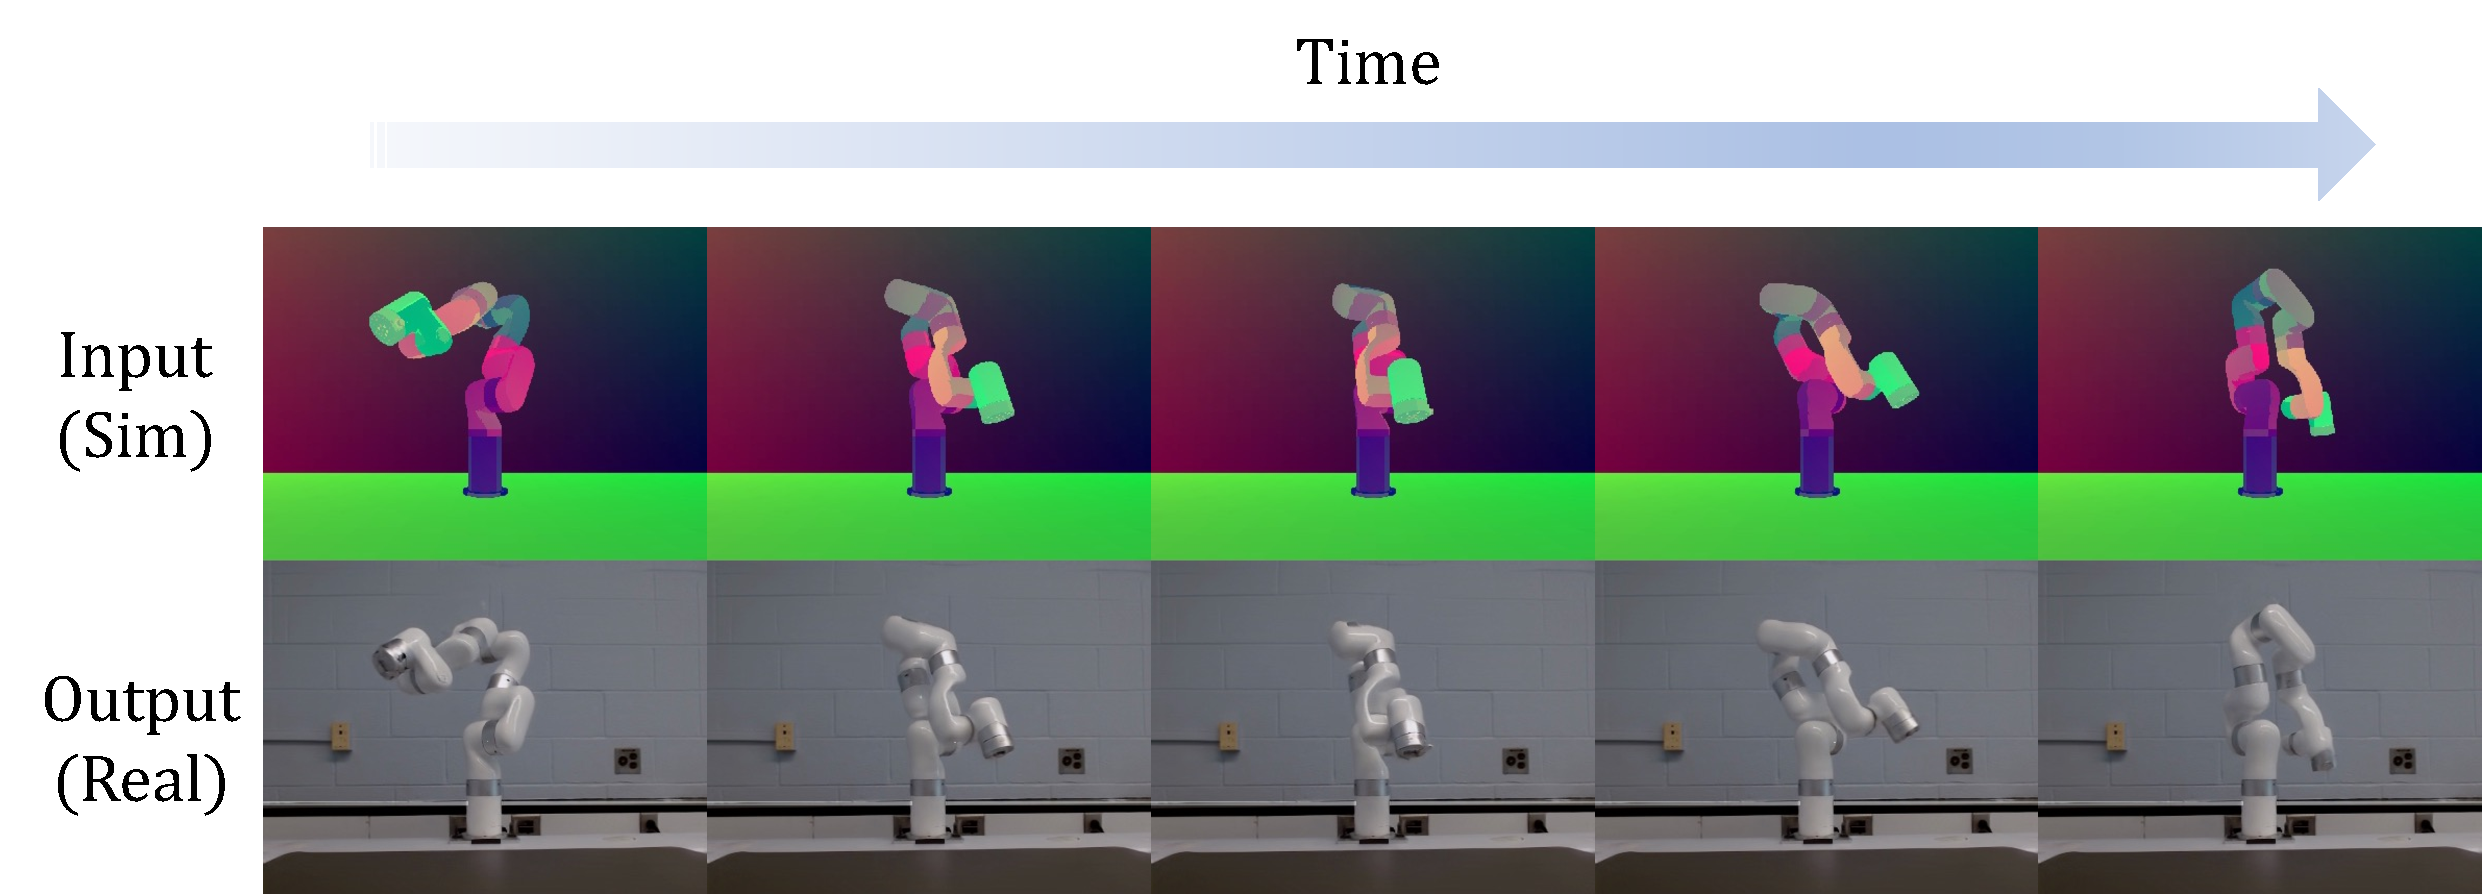
\includegraphics[width=\textwidth]{../images/figure0.pdf}
	\end{center}
	\vspace{-5pt}
	\caption{
		TRITON is a sim-to-real algorithm that makes simulated scenes look realistic. As a black-box, the only input needed is an RGB image shown in the top row, which generates the output on the bottom row.
	}
	\label{fig:figure0}
	\vspace{-5pt}
\end{figure}


Current sim2real image translation algorithms used for robotics \cite{retina_gan,rl_cyclegan} often have difficulty generating consistent results across large time-frames particularly when the objects in an environment are allowed to move. This makes training good robotic policies using such sim2real challenging.
In this paper, we discuss an algorithm called TRITON (Texture Recovering Image Translation Network) that combines neural rendering, image translation, and two special surface consistency losses to create surface-consistent translations.
We use the term surface-consistent to refer to the desirable quality of preserving the visual appearance of object surfaces as they move, or are viewed from another angles. 

TRITON is applicable when we have a simulator capable of generating a realistic distribution of geometric data, but when we do not have any information about the surfaces of those objects (which we need to render realistic images). For example, in our experiments we use a robotic arm model provided by the manufacturer that contains no material information, and then learn to render the materials of the arm using TRITON.
As opposed to requiring an artist to create 3d models with meaningful textures, TRITON can generate these from scratch using a set of photographs capturing the distribution of states in a simulation, without requiring any matches between domains. 
% TRITON is robust to small camera variations, and can recover crisp textures even if the geometry isn't perfect. 

% The three main technical contributions of this paper are our neural neural texture, and two separately sufficient surface consistency losses.
One of the main contributions of this paper is our `neural neural texture'.
Inspired by previous works, TRITON uses raster-based neural textures to create realistic images \cite{deferred_neural_rendering,surgical_video_translation}.
Unlike those works however, we do not use a pixel-based neural texture. Instead, we use what we call a ``neural neural texture'': a continuous implicit pixelless parametric texture represented by a neural netork using fourier features \cite{fourier_feature_networks} that takes in 2d UV coordinates and outputs colors.

We conduct multiple experiments to confirm TRITON's advantage over prior image translation approaches commonly used for sim2real including CycleGAN~\cite{cyclegan} and CUT~\cite{cut}.
%First, we train it on a dataset with alphabet blocks, then compare photographs in that dataset to TRITON outputs by manually aligning the simulated 3d cubes with the photographs.
Important, we show the advantages of the proposed approach in real-robot sim2real experiments, learning the textures and training a robot policy solely based on the images generated by TRITON. 
%We also perform a robotic experiment, where we learn a policy completely in a simulation, and then verify it in the real world. In both of these tests, TRITON outperforms other image translation algorithms. 

\begin{figure}[thbp]
	\vspace{-10pt}
	\begin{center}
		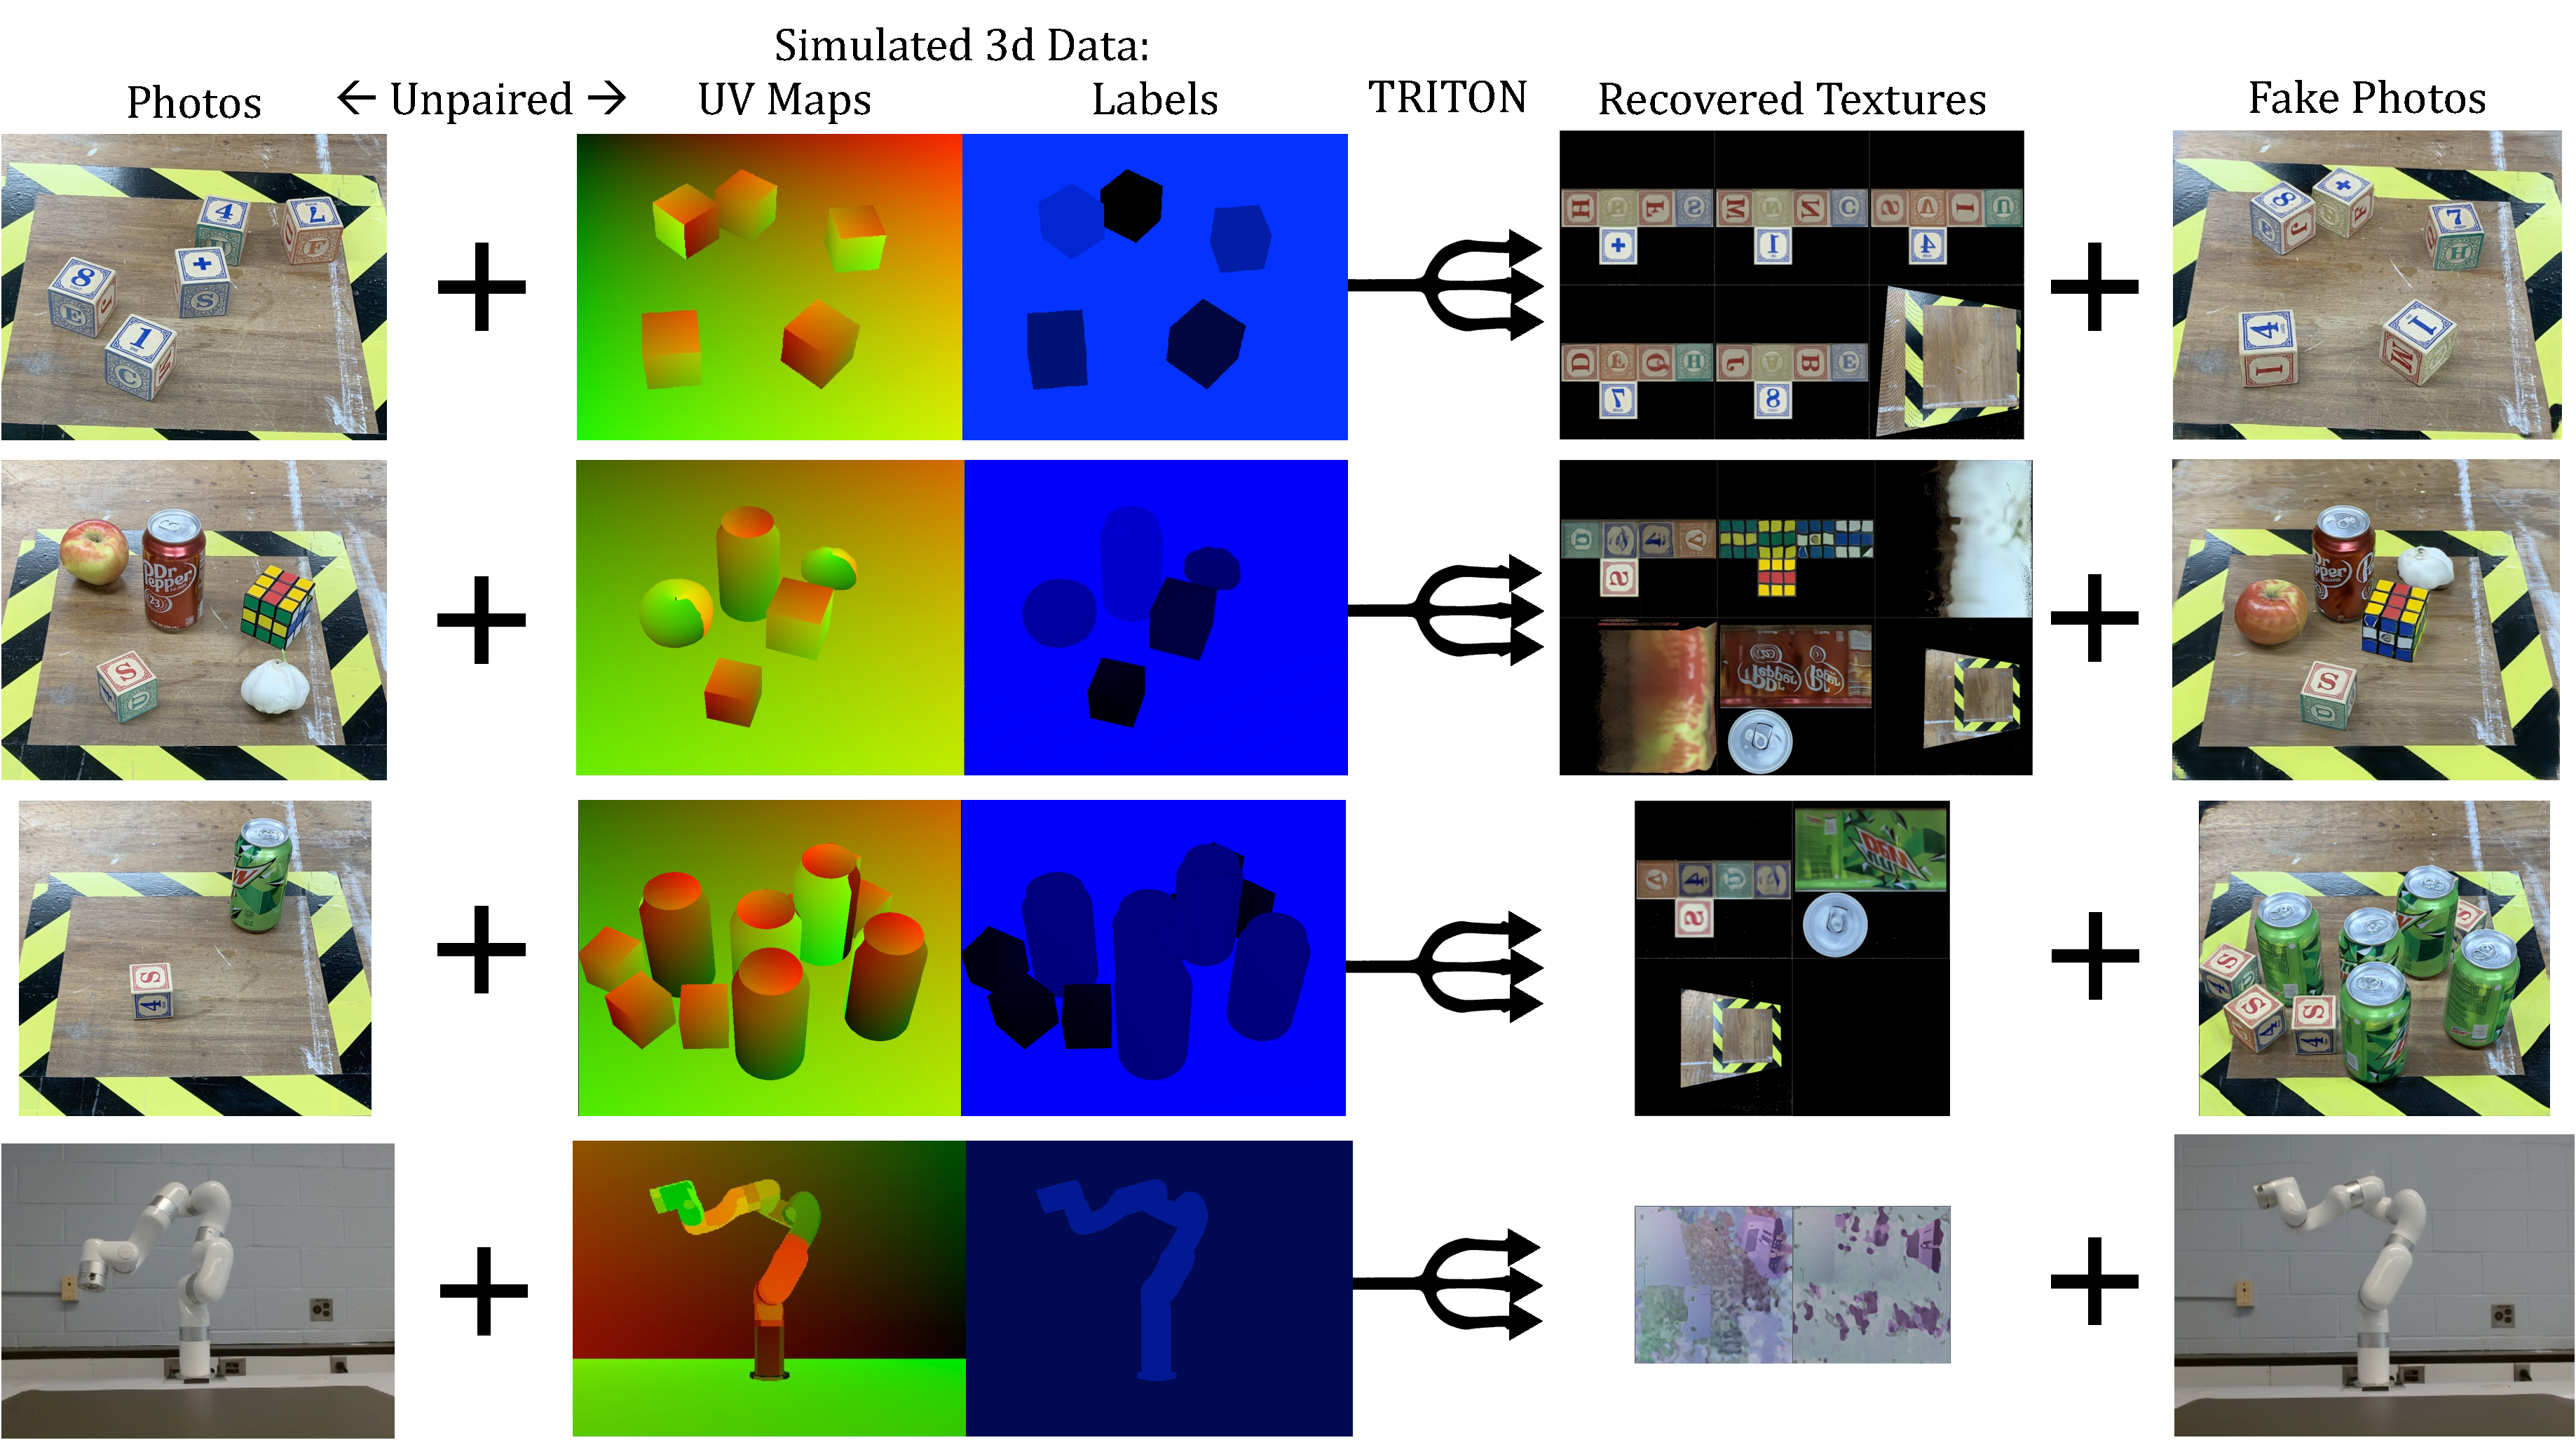
\includegraphics[width=\textwidth]{../images/first_diagram.pdf}
	\end{center}
	\vspace{-5pt}
	\caption{
		This is an overview of what TRITON accomplishes.
		TRITON learns the textures of 3d objects to help translate simulated images into photographs. It does this with unpaired data. Each row is a different dataset.
	}
	\label{fig:first_diagram}
	\vspace{-5pt}
\end{figure}
	
\vspace{-5pt}	
\section{Related Works}
\vspace{-3pt}
\paragraph{Unsupervised Image to Image and Video to Video Translation}
Generative models have been very successful in creating images unconditionally~\cite{gan,stylegan}, creating images conditioned on text~\cite{dalle,imagen} and creating images when trained on paired data~\cite{pixtopix}.
Generative models that translate images between unpaired data is a challenging task as well, but has been done before~\cite{dual_diffusion,cyclegan,munit,unit}.
Of particular interest are sim2real image to image translation algorithms such as~\cite{retina_gan,rl_cyclegan,surgical_image_translation,enhancing_photorealism_enhancement}. These algorithms aim to translate simulated images into realistic ones, for various purposes such as data augmentation or video game enhancement. In particular, \citet{retina_gan,rl_cyclegan} are used to help train robots. Our paper uses an architecture based on~\citet{surgical_image_translation}, which is based on MUNIT~\cite{munit}.
This area of research has been extended to video to video translation, where optical flow is often used to create a stateful translation where temporal coherence is preserved~\cite{tecogan,mocyclegan}. These algorithms fail to provide temporal coherence over long time periods, however. Another work from~\citet{surgical_video_translation}, is closely related to ours and uses neural rendering to translate videos with temporal coherence even when the camera spins around all the way.

\vspace{-8pt}
\paragraph{View Synthesis}
View synthesis is a field of research where we predict the outputs of unseen camera viewpoints. NeRF \cite{nerf} has spawned a large body of research on end to end view synthesis, resulting in works such as \cite{nerv,fast_nerf,barf}. Related to our work, which also uses geometry based backbone are \cite{free_view_synthesis,stable_view_synthesis,ners}. All of these works, however, only work with static scenes. There are NeRF-based approaches that work on dynamic scenes \cite{dnerf,nerfies,nerualradianceflow} but none of these interactive. \citet{playable_environments} is interactive, but its conditioned on learned actions and not compatible with physics simulators that would be used to train robots.

\vspace{-8pt}
\paragraph{Neural Textures}
\citet{deferred_neural_rendering} introduced the concept of neural textures and image translators in the context of a deferred rendering pipeline, used in other works such as \cite{surgical_video_translation} which is closely related to our project. 
\citet{surgical_video_translation} differs from TRITON in a few very important aspects though, the biggest being that it only synthesizes new camera views, where the only difference between each scene is the placement of the camera. In contrast, our algorithm takes in scenes where several objects are placed in different places or deformed, so that one static  global 3d model of the environment is not sufficient to accomplish our tasks. In addition, TRITON uses a new type of neural texture called a ``neural neural texture'', which is represented continuously using a fourier feature network, as described in \citet{fourier_feature_networks}.

% Problem: 
% Why is this problem important?
% No view consistency.

% Introducing our intuition of what improvements can solve this problem.

% Our exact method - introducing our components and what we're doing

% Conclusion: This works well, and our contributions are x

% I introduce you to TRITON. The rest of the introduction text goes here; I've commented out my old incomplete introduction.







	% TODO: Note that the simple input of UVL, or an RGB neural texture, means any simulator should be plug-and-play with this algorithm.

	% Recently, several sim-to-real algorithms have come out that are based on image-to-image translation. [Citations]
	% These are used for training robots using pixel-based reinforcement learning.
	% They demonstrated that better image translation algorithms yielded notable improvements in robotic benchmarks.
	% At the same time, there is a lot of research on differentiable rendering,
	% a topic which produced papers such as NERF which attempt to capture 3d representations of the real world.
	% However, most of these approaches are either supervised or involve only camera movements [citations].
	% One paper that came out recently combined both image translation and differentiable rendering in an unsupervised manner to create view-consistent models of human organs [citation].
	% This paper too, though, was limited to only camera movements.

	% This algorithm unlocks a new capability: learning textures to match photos for given 3d models without supervision.

	% The motivation for this paper is to create a temporally consistent sim-to-real image translation algorithm that will look the same from multiple camera angles simultaneously, keeps all semantic details 
	% [[I'll finish this later... let's work on the meat of the paper first...]]

%===============================================================================
% \vspace{-5pt}
\section{Formulation}
\label{sec:data}
\vspace{-3pt}
	% TRITON stands for Texture Recovering Image Translation Network. It has two goals: to translate images, and to recover textures.
	TRITON's goal is to turn 3d simulated images into realistic fake photographs (by training it without any matching pairs), while maintaining high surface consistency.
	It does this by simultaneously learning both an image translator and a set of realistic textures.
	These translations can be useful for downstream tasks, especially robotic policy learning from camera data, enabling sim2real.
	
	In contrast to previous works involving ``neural textures'' \cite{deferred_neural_rendering,surgical_video_translation}, TRITON can handle more than just camera movements:
	the positions of objects in the training data can be moved around or deformed as well between data samples.
% 	For this reason, we chose the term ``surface consistency'' instead of ``view consistency'', which was the term used in [] \textbf{(mryoo: cite)}.
	With high surface consistency, surfaces of translated objects will look the same even when moved around or viewed from different camera angles.

	\begin{figure}[H]
	    \vspace{-5pt}
		\begin{center}
			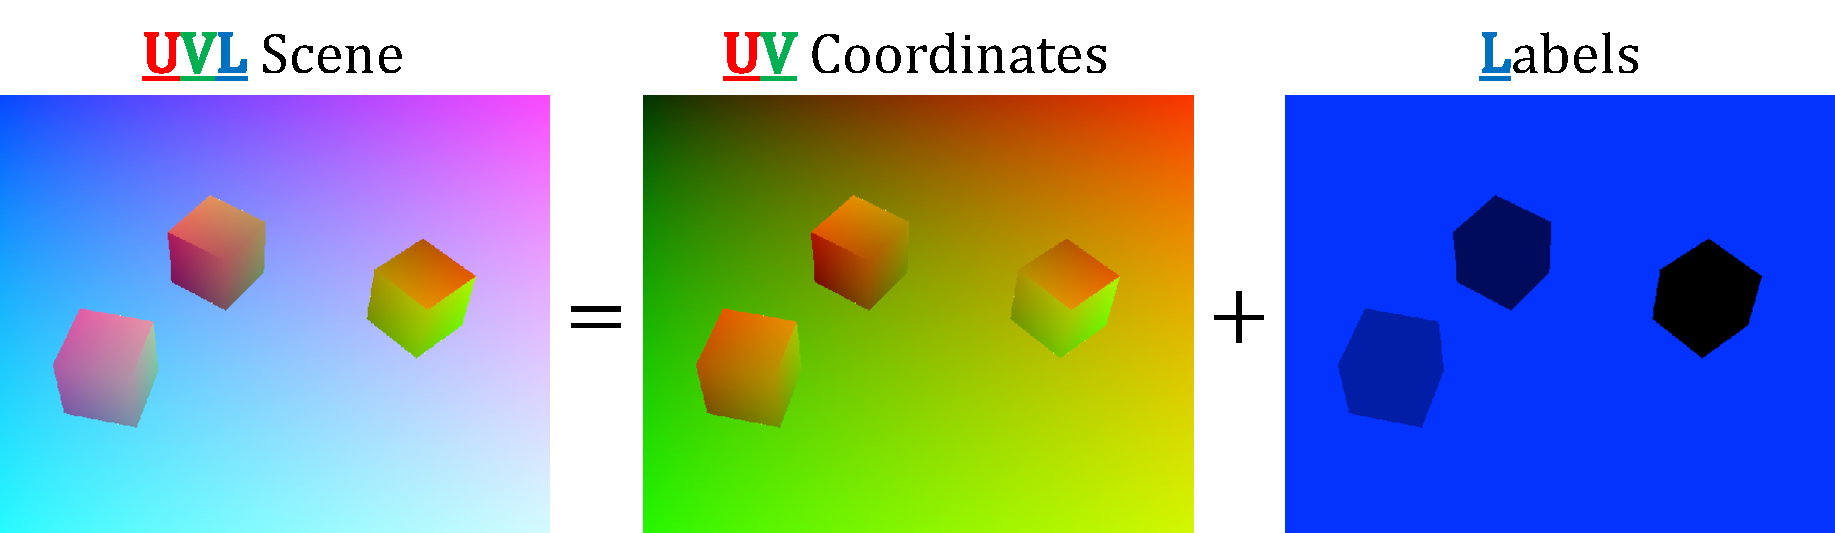
\includegraphics[width=.8\textwidth]{../images/uvl_explanation_minimal.pdf}
		\end{center}
		\vspace{-10pt}
		\caption{
			A scene is obtained by rendering a 3d state into an image, where the first two color channels represent $u,v$ coordinates and the third channel $l$ represents object labels.
			% This diagram shows the purpose of a UVL image.
			% A UVL scene is an image that has three channels: RGB.
			% R and G are used for U and V, and B is used for L.
			% L stands for Label, and determines which part of the synthetic image will get which texture.
			% The U and V coordinates correspond to positions on each texture,
			% telling it how to project the textures onto the 3d objects represented in the UVL scene.
			% The darkest shade of blue corresponds to the 1st texture, and the next darkest shade of blue corresponds to the 2nd texture etc.
			}
		\label{fig:uvl_explanation}
		\vspace{-15pt}
	\end{figure}

	There are two components in every dataset: A set of simulated 3d scenes, and a set of photographs.
	Datasets usually have many more scenes than photographs, since scenes can be generated automatically.
	% The photographs, having $(r,g,b)$ values between 0 and 1,
	% 	are denoted as $p \in [0,1]^{N \times 3 \times H \times W}$ where $N$ is the batch size,
	% 	3 refers to the three $(r,g,b)$ channels, 
	% 	and $H,W$ are the height and width respectively.
	% A photograph in a set of photographs, having $(r,g,b)$ values between 0 and 1,
	% 	is denoted as ${p^n \in [0,1]^{ 3 \times H \times W}}$ where $n$ is that photograph's index in that set,
	% 	3 refers to the three $(r,g,b)$ channels, 
	% 	and $H,W$ are the height and width respectively.
	A photograph is an image tensor, having $(r,g,b)$ values between 0 and 1,
		is denoted as ${p \in [0,1]^{H \times W \times 3}}$ where 
		3 refers to the three $(r,g,b)$ channels, 
		and $H,W$ are the height and width respectively.
		
	In this work, a scene refers to a rendered 3d simulation state - which includes the position, rotation, and deformation of every object (including the camera).
	% Using some 3d rendering software, be it Blender or Gazebo or some other 3d creates an image from these 
	We represent each 3d state with a simple $(r,g,b)$ image, in a simple enough format that any decent simulator should able to provide.
	% These have the same datatype and dimensions as photographs and are denoted as 
	% $s \in [0,1]^{N \times 3 \times H \times W}$.
	% A scene has the same dimensions as a photograph and is denoted as 
	% $s^n \in [0,1]^{3 \times H \times W}$.
	A scene has the same dimensions as a photograph and is denoted as 
	$s \in [0,1]^{H \times W \times 3}$.
	However, unlike $p$, $s$'s three $(r,g,b)$ channels encode a special semantic meaning: $(u,v,l)$ as depicted in Figure \ref{fig:uvl_explanation}.
	The channels $u$ and $v$ refer to a texture coordinate, whereas $l$ refers to a label value that identifies every object in a scene.
	In a given dataset, each object gets a different label. Likewise, each object is assigned a different texture.
	We assume that every dataset has $L$ different label values, $L$ different objects, and that we must learn $L$ different neural textures.
    % TODO: Say I scales and discretizes l, don't say more than that. 
% 	In each dataset, we must also define a function $I(l)$ that maps label values to texture indices. A simple way to do this is with the following definition:
% 	\begin{equation}
% 		I: \left\{\frac{1}{L},\frac{2}{L},\dots \frac{L}{L}\right\} \rightarrow \left\{1,2,\dots L\right\}  \eqand  I(l)=l\cdot L
% 	\end{equation}
% 	However, this mapping can be changed arbitrarily if its more convenient to do so for a given dataset.
% 	Also please note that this paper uses 1-based indexing for notational simplicity. 




	% TODO: Describe what UVL is ; 
	% Formulate the setting: What our inputs are and the targets are and what we learn (a neural texture function) and how we can take advantage of it for robotic learning.
	% Don't go into details; just say 'its a black box function'

	% TODO: Add UV to the fourier feature diagram.

	% TODO: Create subfigures with subcaptions. 
	% 2a: Nothing but UVL=UV+L
	% 2b. 3d uvl axis to texture pack (drew on whiteboard)
	% 2c. Skip over the translation network and show a pretty robot arm picture

	% This is the formulatoin section; not data section. Dont talk about how many photos we use etc. 

	% JUST IN CASE THINGS ARE ERASED:
	% We learn neural texture corresponding to each object, where each texture is represented as a function mapping... 
	% The idea is to learn object textures as a set of continuous functions from a set of (unlabeled) real images, and use them to generate realistic images.
	% Given a 3D structure of the scene represented with a UVL image, the learned neural textures will translate them into a realistic image.
	% When used for the robot learning, this enables learnable, realistic sim2real of robot training images.

	% IN THE INTRODUCTION: How we're using a neural neural network network texture. Also in related works.

	% TODO: Replace neural texture in figure 3 with axis, and treat it as a function that takes UV in with an arrow pointing to it.

	% BREAK IT DOWN APPROACH:
	% Don't have any pictures. Have breakdown where we add new things in multiple figures.
	% First figure: Just image translation. 
	% Seconf:
	% Third:
	% Etc...


	% In this paper, we'll mostly focus on a hand-collected dataset that involves three alphabet blocks that are moved across a table.
	% Alphabet blocks were chosen because they all have the same geometry (a cube), but have very distinct semantic textures that will make temporal inconsistency obvious to the human eye.
	% This dataset is analogous to data that would be collected for a third-person robotic grasping task.
	% However, other objects (such as cans of soda, apples, cloves of garlic, etc) are also for generating other results in this paper. ((TODO: Detail the five object tests and five cube tests and other stuff like shiny cans etc)).

	% There are two components to this dataset: Simulated data in the form of UVL scenes, and photographs.
	% The camera in the simulation is positioned in approximately the same place as the real camera, with approximately the same field of view.
	% In both domains of this dataset, the camera never moves. Instead, the objects are randomly positioned and rotated on the table.
	% In both the simulation and in real life, these objects are randomly translated along the x and y-axis of the table, as well as rotated on the z-axis.

	% There are 200 photographs in this dataset, and they are recorded as RGB jpg images.
	% There are 3000 synthetic images in this dataset, in the form of UVL images.
	% These UVL images are also encoded as RGB images, but provide information about the geometry of a scene.
	% UVL images are composed of both a UV map and a label map and are summarized in figure \ref{fig:uvl_explanation}.
	% To avoid positional rounding errors, UVL images are encoded as EXR files: an image format that supports floating-point values.

	% The pixels in a UVL image are visualizable in RGB space because, like RGB images, each pixel is a vector with 3 values. The first two channels, U and V, are floating point values between 0 and 1. The L channel is also a floating point value between 0 and 1, it has a second meaning. There are only a finite number of label values (corresponding to the number of learnable textures). The rank of a particular L value is used to index these textures.

	% In the three-cube dataset we have 4 textures, and UVL scenes contain label values $l \in [\frac{0}{3}, \frac{1}{3},\frac{2}{3}, \frac{3}{3}]$. A pixel in a UVL scene $l=\frac{2}{3}$ will get indexed to the third texture, because $\frac{2}{3}$ is the third smallest label value.

	% Domain A and B
	% p hat
	% s hat

% %===============================================================================
\vspace{-8pt}
\section{Method} \label{sec:method}
	\begin{figure}[thbp]
	    \vspace{-15pt}
		\begin{center}
			% \includegraphics[width=400pt]{../images/main_diagram_condensed.pdf}
			% \includegraphics[width=400pt]{../images/main_diagram_condensed_with_domains.pdf}
			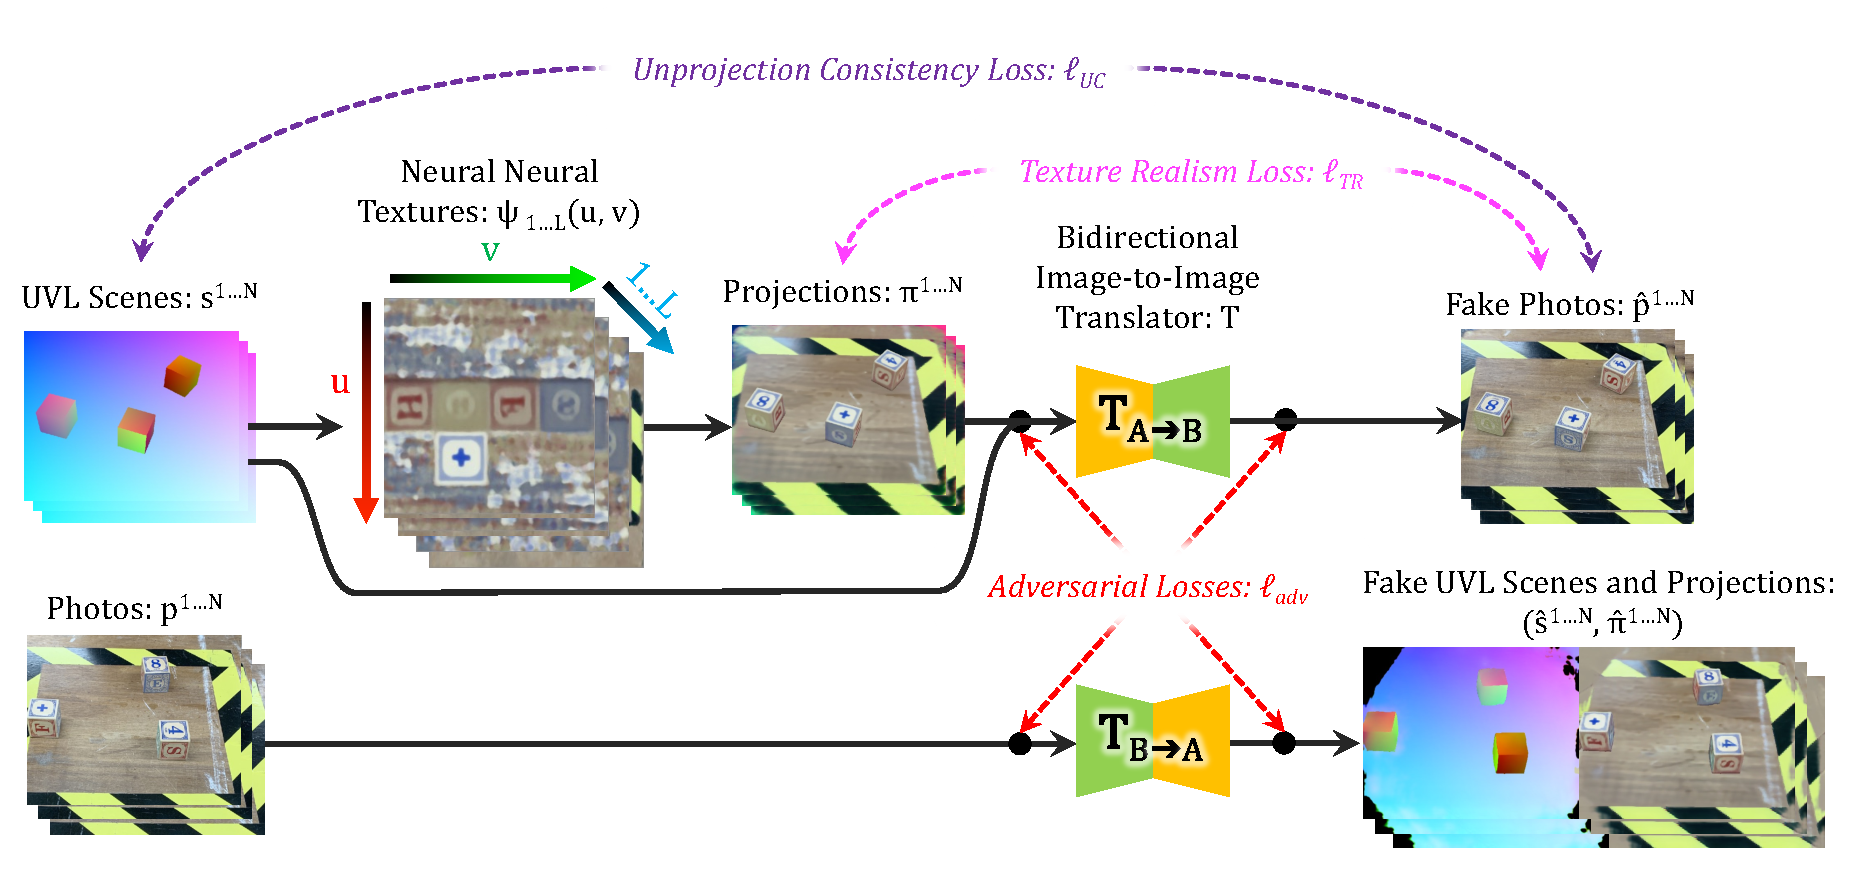
\includegraphics[width=0.9\textwidth]{../images/main_diagram_beautiful.pdf}
		\end{center}
		\vspace{-10pt}
		\caption{
			% We use differentiable rendering paired with unpaired image translation to consistently= transform synthetic scenes into realistic images.
			% To ensure all objects look consistent in different positions and views, we learn the albedo of each object's surface by using a learnable latent texture.
			% This texture is parametrized as an image generated by an MLP which is fed Fourier features, as shown in figure \ref{fig:learnable_textures}.
			% $N$ is the batch size, and $L$ is the number of different labels (which is also the number of learnable textures).
			%
			%JUNE 12:
			%Don't say 4 main components; say 2 components and 2 losses
			%TODO: Try to use right-angled arrows
			%TODO: Use tau as a function
			%Copy paste the figure multiple times, deleting things
			%Mention "Neural Neural Texture": Its a function mapping UV to RGB
			%Formulation doesnt mentino texture; just uvl inputs and final outputs
			%Always use function notation tauuv instead of just tau (in figure as well) 
			%The arrow should be running through tau. It's not a variable its a function...
			%Rename 'B' to "N" for batch size
			%Figure 8: Align consistent with inconsistent and use all 5 green ones
			%
			This figure is an overview TRITON.
			Inputs are on the left, and outputs are on the right.
			The dashed arrows indicate losses.
			Although $\pi\toN$ and $\ph\toN$ look similar, they are not identical - $\lTR$ encourages them to look as similar as possible.
			% $\pi$ is simply projected textures, whereas $\hat{p}$ has been run through an image translator, allowing it to have shadows and specularities.
			% TODO: Come up with a tour of this diagram in this caption. Also maybe make it larger?
			% TODO: Use variables instead of 3,4
			% TODO: Make the text larger and easier to read
			% TODO: Simplify the diagram?
		}
		\label{fig:main_diagram}
	\end{figure}
		In this section, we describe how TRITON works to translate images from domain A (simulation) to domain B (photos) while maintaining surface consistency. 
		TRITON introduces a learneable neural neural texture with two novel surface consistency losses to an existing image translator. In the end, TRITON is able to effectively generate photorealistic images.
		%JUNE 12:
		%TODO: MIgrate all four of these teasers into their respective subsections to save space.
\vspace{-3pt}
	\subsection{Neural Neural Texture Projection}
	\label{sec:neural_tex}
	\vspace{-3pt}
		\begin{figure}[t]
		    \vspace{-5pt}
			\begin{center}
				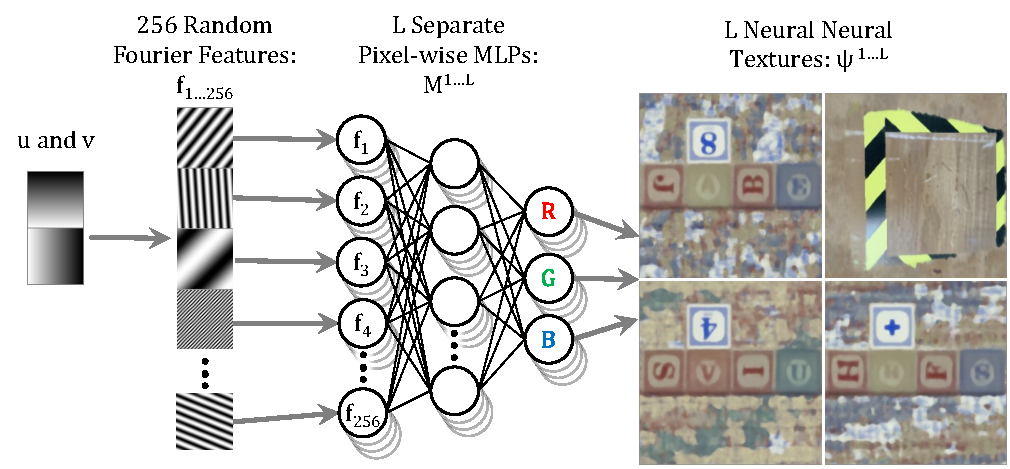
\includegraphics[width=0.8\textwidth]{../images/learnable_textures.pdf}
			\end{center}
			\vspace{-3pt}
			\caption{
				This figure details how our neural neural textures are calculated in Figure~\ref{fig:main_diagram}. They are fully differentiable, and represented continuously along the texture's u and v axes using Fourier feature networks.
			}
			\vspace{-3pt}
			% For each texture, there is a separate Fourier feature network (Fourier features fed into a pixel-wise MLP) that will take in Fourier features as inputs, and output an RGB image using the method described in \citet{fourier_feature_networks}.
			% We found this method gave better results than storing each differentiable texture as a raster matrix of pixels, as well as being faster to train.
			% During inference, you can store the results of this MLP as a raster image of arbitrarily large resolution, saving both time and VRAM.
			\label{fig:learnable_textures}
		\end{figure}

		%JUNE 12:
		%Defining what it is and how it's used.
		%
		%Justify why we're calling it neural neural texture. Unlike previous papers [citations], we learn a neural network instead of a grid of pixels. To be explicit we call it neural neural texture. %%%%%% Previous papers were more like latent textures but ours is different: it is a funciton.  Previous works were called "Neural Textures" but we're going to call ours "Neural Neural Textures" - a subtype of neural textures. 

		% Using neural neural textures, we can encode features directly onto the surfaces of the 3d objects in a scene, which the image translation module uses to maintain visual consistency between states and viewpoints.
		Instead of feeding a scene $s$ directly into the image translator $\Tab$, we first apply learnable textures $\psi$ to its surfaces as shown in Figure \ref{fig:main_diagram}.
		Previous works called these learnable textures ``neural textures'', and were parametrized by a discrete grid of differentiable texels. 
		% In contrast, we call our learnable textures ``neural nerual textures'', becuase our textures are a type of neural texture that is parametrized continuously over UV space using a neural fourier feature network.
		In contrast, we call our learnable textures as ``neural nerual textures'', because our textures themselves are represented as a neural network function, parameterized continuously over UV space.
		Our neural textures $\psi\toL$ are learned jointly with our image translator $T$.
		
		These neural neural textures are represented implicitly by a neural network that maps UV values to RGB values. %, and are used to obtain projections $\pi$ from 3d scenes $s$.
		For each texture $\psi^i \in \psi\toL$, 
		\begin{equation}
			\psi^i: (u,v) \in\real^2 \rightarrow (r,g,b) \in\real^3 % \eqand 
		\end{equation}
		Given a scene $s$, we obtain projection $\pi$ by applying a texture $\psi^i \in \psi\toL$ to every pixel $(u,v,l) \in s$ individually, where texture index $i=I(l)$ is decided by the label value $l$ of that scene pixel.
		% Each pixel in the resulting projection $rgb\in\pi$ is the result of selecting a texture index $i$ based on the rank of label value $l$, then applying $\psi^i$ to the $u,v$ values.
		\begin{equation}
			% \pi=\psi\toL(s) \eqand rgb \in \pi = \psi^i(uv)
			% \pi_{n,c,x,y}=\psi^i(s_{n,1,x,y},s_{n,2,x,y}) \eqwhere 1\le n\le N,\ \  1\le c\le 3 ,\ \ 1\le x\le W,\ \ 1\le y\le H,\ \ \text{and} \ \ i=I(s_{n,3,x,y})
			% \pi_{n,c,x,y}=\psi^i(s_{n,1,x,y},s_{n,2,x,y})
			\pi_{[x,y]}=\psi^i(s_{[x,y,1]},s_{[x,y,2]})
		\end{equation}
		% where $1\le n\le N,\ \ 1\le c\le 3 ,\ \ 1\le x\le W,\ \ 1\le y\le H,\ \ \text{and} \ \ i=I(s_{n,3,x,y})$.
		% where $n\in \{1\dots N\},\ \ c\in \{1\dots 3\} ,\ x\in \{1\dots W\},\ y\in \{1\dots H\},\ \ \text{and} \ \ i=I(s_{n,3,x,y})$.
		where $ x\in \{1\dots W\},\ y\in \{1\dots H\}$. Texture index $i = I(l)$ where $l=s_{[x,y,3]}$ and the function $I(\cdot)$ scales and discretizes $l$ into integers. Subscripts mean multidimensional indexing.

		%DISCARDED TEXT:
		% A particular neural texture $\psi^i$ uses maps $uv \rightarrow rgb$. Similarly, the set of textures $\psi_{1\dots L}$ maps uvl values to rgb values: $\psi_{1\dots L}(uvl)=\psi_l(uv)$ where $uvl$ is the concatenation of a $uv$ vector with a label $l \in 1\dots L$.
		% TRITON's neural neural texture module lets it create features on the surfaces of objects, and thus take advantage of 3d geometric priors. 

		
				% The neural texture applied to a particular scene pixel $uvl \in s$ is multiplexed by $l$, and the respective output pixel $rgb \in \pi = \psi_luv$. 
				% Texture projections $\pi$ are obatined by applying a set of $L$ different neural neural textures $\psi\toL$ to a UVL scene $s$ pixelwise.
				% [[IMPORTANT: THIS IS TECHNICALLY INCORRECT AS l IS A VALUE BETWEEN 0 and 1]]
				
				
				% where $i\in[1,L]\cap\mathbb{Z}$ is the rank of $l$
				% When applied to a UVL scene, it is applied to each $uvl \in s$ pixel individually where every pixel $rgb \in \pi = \psi$ 
				%What is it...then how do we use it...
				% (as the 2nd sentence)
				% Given a 3D scene $s$, we apply $\psi\toL$ to each UV to obtain RGB surface values...
				% project learnable RGB textures $\psi\toL$ to their surfaces to obtain projection $\pi$. 
				% 			Neural Neural Textures $\psi\toLuv$: Given an input scene $s$ depicting 3d objects with labels $1\dots L$, we apply a function on their surface's UV values with neural textures $\psi\toL$ to obtain projection $\pi$.
				
				% \begin{equation}
					% \pi=\psi\toL(s)
				% \end{equation}
				%


		%THIS WILL BE REPLACED BY SUMMARY SECTION
		% 	Given a batch of $N$ UVL Scenes $s_{1\dots B}$ with $L$ different label values, we project $L$ different neural textures $\psi_{1\dots L}$ onto that scene; obtaining projections $\pi_{1\dots B}$. This projection mechanism is illustrated in figure \ref{fig:uvl_explanation}.
			
		% Each neural texture $\psi^i$ is a function consisting of two components: a multi-layer perceptron $M^i$ and a static set of 256 random spatial frequencies $f_{1...256}$. 
		% Given a two-dimensional $uv$ vector, the spatial frequencies are used to generate a high dimensional embedding used as input for the MLP.
		% \begin{equation}
		% 		\psi^i(uv) = 
		% 		\
		% 		M^i\left(\left[
		% 			\sin \left( f_1     \cdot \left(u,v\right) \right) , \ 
		% 			\cos \left( f_1     \cdot \left(u,v\right) \right) , \ 
		% 			% \sin \left( f_2     \cdot \left(u,v\right) \right) , \ 
		% 			% \cos \left( f_2     \cdot \left(u,v\right) \right) , \ 
		% 			\dots \ 
		% 			\sin \left( f_{256} \cdot \left(u,v\right) \right) , \ 
		% 			\cos \left( f_{256} \cdot \left(u,v\right) \right)  \ 
		% 		\right]\right)
		% \end{equation}
		% where $uv$ and $f^i \in N_{ormal}(\mu=0,\ \sigma=10)$ are two dimensional vectors,
		%  $f^i uv$ represents their dot product, 
		% %  $rgb$ represents a 3d color vector,
		%  and $M^i$ maps a $uv$ embedding to an $rgb$ color value:
		%  $M^i: \real^{256} \rightarrow \real^3$.
		% Note that there is nothing special about 256 or 10: these hyperparameter values just happen to work nicely.
		
		We now discuss the implementation of our neural neural networks $\psi\toL$.
		Each neural neural texture $\psi^i$ is a function consisting of two components: a multi-layer perceptron $M^i$ and a static set of 256 random spatial frequencies $f_{1...256} \in \real ^ {256 \times 2}$. 
		Given a two-dimensional $(u,v)$ vector, the spatial frequencies are used to generate a high dimensional embedding of $(u,v)$ as input for $M^i$, where $M^i$ is a function $\real^{256} \to \real^{3}$ mapping that embedding to an $(r,g,b)$ color value:
		\begin{equation}
				\psi^i(u,v) = 
				\
				% M^i(
				% 	\sin( f_1     uv  ) , \ 
				% 	\cos( f_1     uv  ) , \ 
				% 	\sin( f_2     uv  ) , \ 
				% 	\cos( f_2     uv  ) , \ 
				% 	\dots \ 
				% 	\sin( f_{256} uv  ) , \ 
				% 	\cos( f_{256} uv  )  \ 
				% )
				M^i(
					\sin( g_1      ) , \ 
					\cos( g_1      ) , \ 
					\sin( g_2      ) , \ 
					\cos( g_2      ) , \ 
					\dots \ 
					\sin( g_{256}  ) , \ 
					\cos( g_{256}  )  \ 
				)
		\end{equation}
		where $g_k=f_k\cdot(u,v)$
		% , $f^i \in N_{ormal}(\mu=0,\ \sigma=10)$ is a two dimensional random gaussian vector,
		, $f_k \in \mathcal{N}(\mu=0,\ \sigma=10)$ is a two dimensional random gaussian vector,
		\mbox{and $\cdot$} is the dot product operator.
		%  $rgb$ represents a 3d color vector,
		% :
		% $M^i: \real^{256} \rightarrow \real^3$.
		The hyperparamters 256 and 10 are selected empirically.
		%Note that there is nothing special about 256 or 10: these hyperparameter values just happen to work nicely.
		
		
		%Squeeze this down - we don't need explanations for why, that can go in the appendix.
		In practice, we found that TRITON learns faster and more stably with our neural neural textures than it does with raster neural textures. The generated textures are also smoother and less noisy. See the supplementary material for more details.
		% The trained fourier-feature textures also exhibit less noise than its raster counterparts. 
		% We think this is because they do not suffer as much. 
		% It cfrom aliasing artifacts in the UV maps, where the loss gradient might skip over pixels in texture-space when the UVL scene is zoomed out too far or raster resolution is too high. 
		% Case in point: if you have a raster texture with very high resolution, the loss gradient is less likely to be passed to a given texel because the chance that a given UV value in a scene will be rounded to that pixel's coordinates is very small.

		% UV Map projection
		% We use an RGB texture, parametrized by an MLP taking fourier features as an input.
		% We use a separate MLP for every texture. 



\vspace{-3pt}
	\subsection{Image Translation}
	\label{sec:image_translation}
\vspace{-3pt}
	% 	\begin{figure}[H]
	% 		\begin{center}
	% 			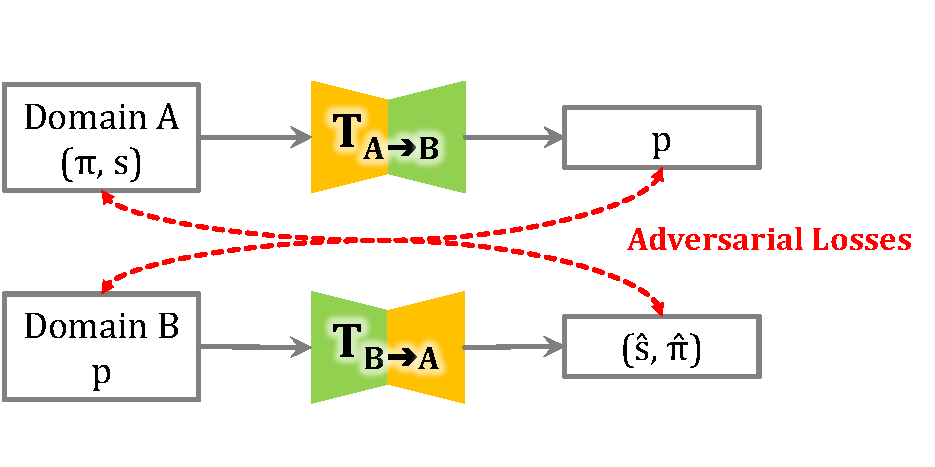
\includegraphics[width=200pt]{../images/module_translator.pdf}
	% 		\end{center}
	% 		\caption{
	% 			A subset of figure \ref{fig:main_diagram} focusing on the image translation module $T$.
	% 		}
	% 		% For each texture, there is a separate Fourier feature network (Fourier features fed into a pixel-wise MLP) that will take in Fourier features as inputs, and output an RGB image using the method described in \citet{fourier_feature_networks}.
	% 		% We found this method gave better results than storing each differentiable texture as a raster matrix of pixels, as well as being faster to train.
	% 		% During inference, you can store the results of this MLP as a raster image of arbitrarily large resolution, saving both time and VRAM.
	% 		\label{fig:module_translator}
	% 	\end{figure}


		% TO PUT IN FORMULATION:
		% The simulation domain A (UVL maps concatenated to their texture projections) has 6 channels, whereas the real image domain B (photographs) has 3 channels. An element of A is $\ppis \in A$ and $p \in B$.
		% $p \in B$ is a batch of real photos,
		% and $\ppis\in A$ is a batch of simulated projection/uvl scene concatenations. 

		% TODO: Why doesn't citep work? The references don't show the authors names...it used to work...did I mess up example.bib?

		% TODO: Get rid of the variable "C" and replace it with $\ppis$

		% TODO: Is l2 loss capitalized or lower case?




		%_i
		% Our image translation module $T$ is bidirectional: $\Tab$ translates images from domain A to domain B, and $\Tba$ translates images from domain B to domain A.
		Our image translation module $T$ is bidirectional: $\Tab$ translates sim to real (aka domain A to domain B), and $\Tba$ translates real to sim (aka domain B to domain A).
		\begin{equation}
			\ph=\Tab(\pis)  \eqand  \ppish=\Tba(p)
		\end{equation}
			
		$T$ is based on the image translation module used in \citet{surgical_video_translation}, which is a based on a variant \cite{surgical_image_translation} of MUNIT \cite{munit}. 
		$T$ uses the same network architectures as MUNIT, and also inherits its adversarial losses $\ell_{adv}$, cycle consistency losses $\ell_{cyc}$ and reconstruction losses $\ell_{rec}$.
		The main differences between our image translation model and MUNIT are that we use a different image similarity loss $\Omega$, and like \citet[]{surgical_image_translation} and \citet[]{surgical_video_translation} our style code is fixed (making it unimodal) and noise is injected into the latent codes during training to prevent overfitting. 
		During inference however, this intermediate noise is removed and our image translation module is deterministic. 
		% Apart from these differences, our image translation module has the same loss formulations and generator/encoder/discriminator network architectures as MUNIT. 

		MUNIT translates images by encoding both domains $A$ and $B$ into a common latent space, then decoding them into their respective domains  $B$ and $A$.
		In our translation module, we define fake photos $\ph = \Tab(\pis) = G_B(E_A(\pis))$ and fake projection/uvl scenes $\ppish = \Tba(p) = G_A(E_B(p))$
			where $E_A, E_B, G_A, G_B$ are encoders and generators for domains A and B respectively.
		% We also define the outputs of these translators as fake photos $\hat{p} = T_{A\rightarrow B}(\pis)$ and fake projection/uvl scenes $(\hat{\pi},\hat{s}) = T_{A\rightarrow B}(\pis)$.

		% TODO: Choose one of the three equation representations. Which is best? The next paragraph will look less ugly when the equations are shorter.
		
		% For our purposes, MS-SSIM is a metric that measures the similarity of two BCHW tensors on a scale from 0 to 1.
		% Given two tensors $x$ and $y$, their similarity loss is $\mu\left((x-y)^2\right) - \text{msssim}(x,y)$. 
		We define an image similarity loss $\similar$ between two images $x,y$ that returns a score between -1 and 1, where 0 means perfect similarity:
		\begin{equation}
			\similar(x,y) = L_2(x,y)-\msssim(x,y) 
		\end{equation}
		This function combines mean pixel-wise $L_2$ distance (used in MUNIT) with multi-scale structural image similarity $\msssim$, introduced in \citep{msssim}. Note that this loss can also be applied to the latent representations obtained by $E_A$ and $E_B$, because like images those tensors are also three dimensional.

		% To ensure cycle consistency, we have an image similarity loss $\ell_{cyc}$ to ensure
		% % $c \approx G_A(E_B(G_B(E_A(\pis)))) = T_{B\rightarrow A}(T_{A\rightarrow B}(\pis)) = T_{B\rightarrow A}(\hat{p})$
		% $\ppis \approx T_{B\rightarrow A}(\hat{p})$
		% and vice versa
		% % $p \approx G_B(E_A(G_A(E_B(p)))) = T_{A\rightarrow B}(T_{B\rightarrow A}(\pis)) = T_{A\rightarrow B}(\hat{c}) = T_{A\rightarrow B}(\hat{\pi},\hat{s})$. 
		% $p \approx T_{A\rightarrow B}(\hat{\pi},\hat{s})$.
		% %I only want to use one of the two representations; either using T_AB or GA(EB) etc. Which one should I use?
		% We also impose an image similarity loss $\ell_{rec}$ to ensure that $\ppis \approx G_A(E_A\ppis)$ and $p \approx G_B(E_B(p))$, which is effectively an autoencoder loss. 
		% In addition, we also have content similarity loss $ \ell_{con}$ to make 
		% $E_A(\pis) \approx E_B(\ph)$ and $E_A(p) \approx E_A(\pish)$.
		% % $E_A(\pis) \approx E_B(\Tab(\pis))$ and $E_A(p) \approx E_A(\Tba(p))$.


		We have cycle consistency loss ${\ell_{cyc}  =  \similar\left(\ppis,T_{B\rightarrow A}\left(\hat{p}\right)\right)  +  \similar\left(p,T_{A\rightarrow B}\left(\hat{\pi},\hat{s}\right)\right)}$
		% $\ppis \approx T_{B\rightarrow A}(\hat{p})$
		% and vice versa
		% $p \approx T_{A\rightarrow B}(\hat{\pi},\hat{s})$.
		, similarity loss ${\ell_{rec} = \similar\left(\ppis,G_A\left(E_A\ppis\right)\right) + \similar\left(p,G_B\left(E_B\left(p\right)\right)\right)}$
		%  to ensure that $\ppis \approx G_A(E_A\ppis)$ and $p \approx G_B(E_B(p))$, 
			(which is effectively an autoencoder loss),   
		and content similarity loss ${ \ell_{con} = \similar\left(E_A\left(\pis\right), E_B\left(\ph\right) \right)    +   \similar\left(E_A\left(p\right),E_A\left(\pish\right)\right) }$.
		% $E_A(\pis) \approx E_B(\ph)$ and $E_A(p) \approx E_A(\pish)$.
		We also have adversarial losses $\ell_{adv}$ that come from two discriminators $D_A$ and $D_B$, targeting domains A and B respectively, using the LS-GAN loss introduced in \citet{lsgan}. 
		In total, our image translator loss is $\ell_T=\ell_{cyc}+\ell_{rec}+\ell_{con}+\ell_{adv}$.


		% PRETTIEST BUT TOO MUCH SPACE
		% 		Inheriting from MUNIT, we have three losses: cycle consistency loss $\ell_{cyc}$, content similarity loss $\ell_{con}$, and reconstruction loss $\ell_{rec}$ which functions as an autoencoder loss.
		% 		\begin{eqnarray}
		% \begin{center}
		% 	\begin{align}
				
		% 		\ell_{cyc}  =  \similar\left(\ppis,T_{B\rightarrow A}\left(\hat{p}\right)\right)  +  \similar\left(p,T_{A\rightarrow B}\left(\hat{\pi},\hat{s}\right)\right)
				
		% 		\ell_{con} = \similar\left(E_A\left(\pis\right), E_B\left(\ph\right) \right)    +   \similar\left(E_A\left(p\right),E_A\left(\pish\right)\right)

		% 		\ell_{rec} = \similar\left(\ppis,G_A\left(E_A\ppis\right)\right) + \similar\left(p,G_B\left(E_B\left(p\right)\right)\right)
		% 	\end{align}
		% \end{center}
		% 		\end{eqnarray}


		% In total, the loss for the image translator module $T$ is $\ell_T=\ell_{cyc}+\ell_{rec}+\ell_{con}+\ell_{adv}$.

		% % NOTE: THe other paper \citep{surgical_video_translation} didn't do into this much detail; instead putting most of these losses in teh appendix. I think we can cut this down? I'll check with michael first...right now I'll include everything.


\begin{figure}
    \centering
    \begin{minipage}{0.57\textwidth}
		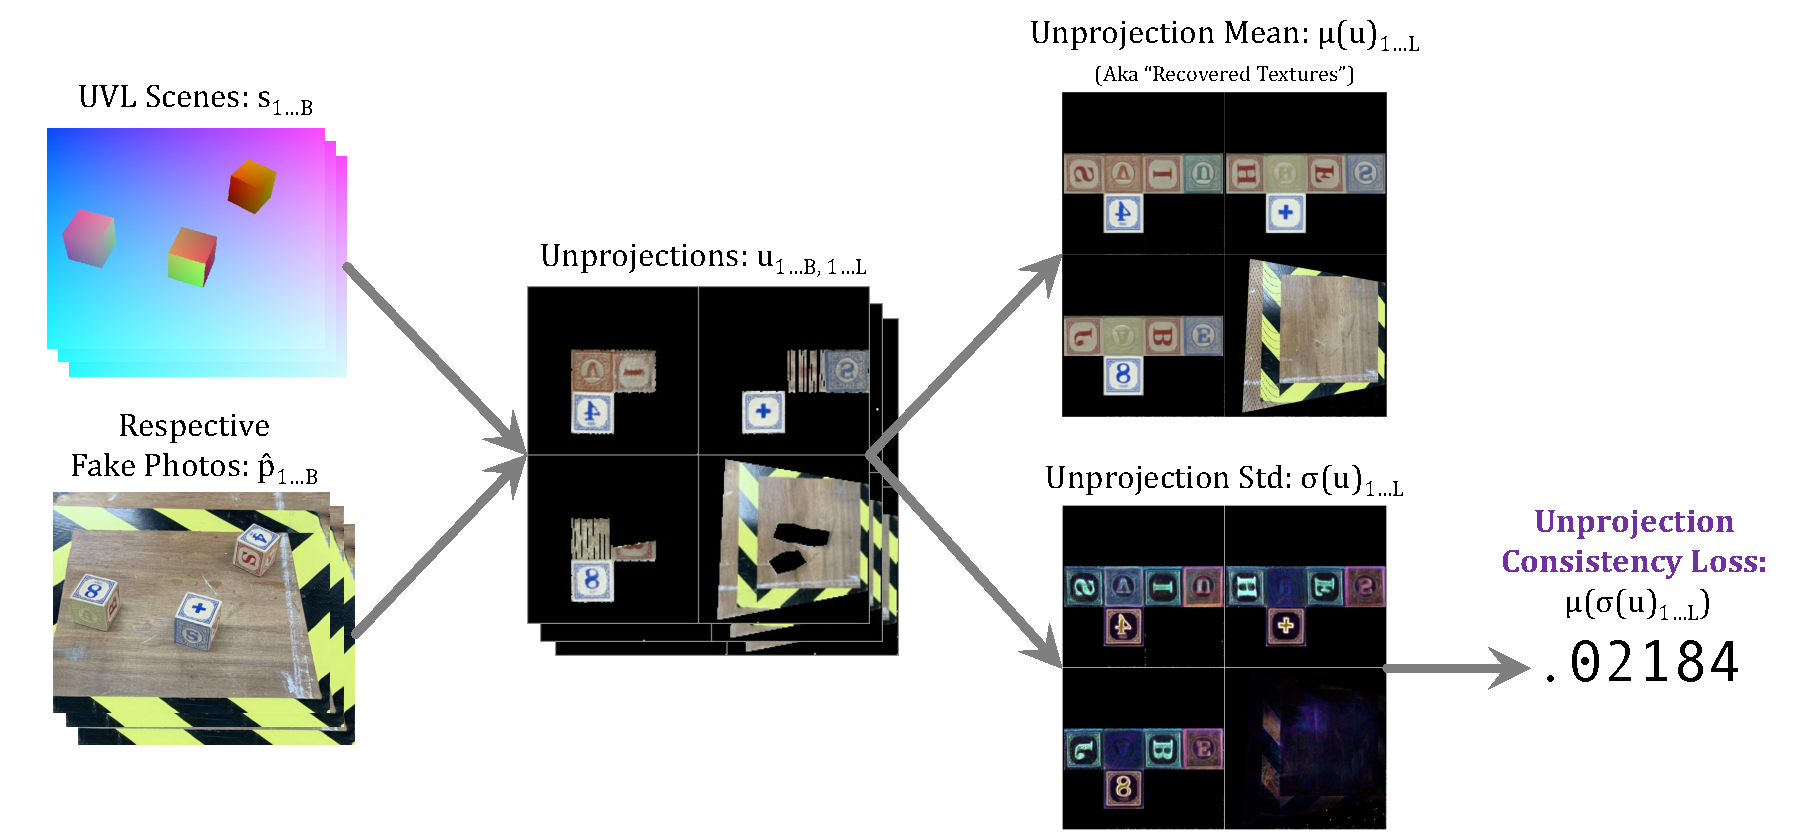
\includegraphics[width=1\linewidth]{../images/unprojection_consistency_loss_without_reprojection.pdf}\label{fig:unprojection_consistency_loss}
		\vspace{-5pt}
	\caption{
		This is the unprojection consistency loss used in Figure~\ref{fig:main_diagram}.
		The Unprojection Mean is not used in any losses, but help to illustrate the content in Section \ref{sec:texture_realism_loss}.
	}
	\end{minipage}
	\hfill
    % \hspace{1cm}
    \begin{minipage}{0.39\textwidth}
        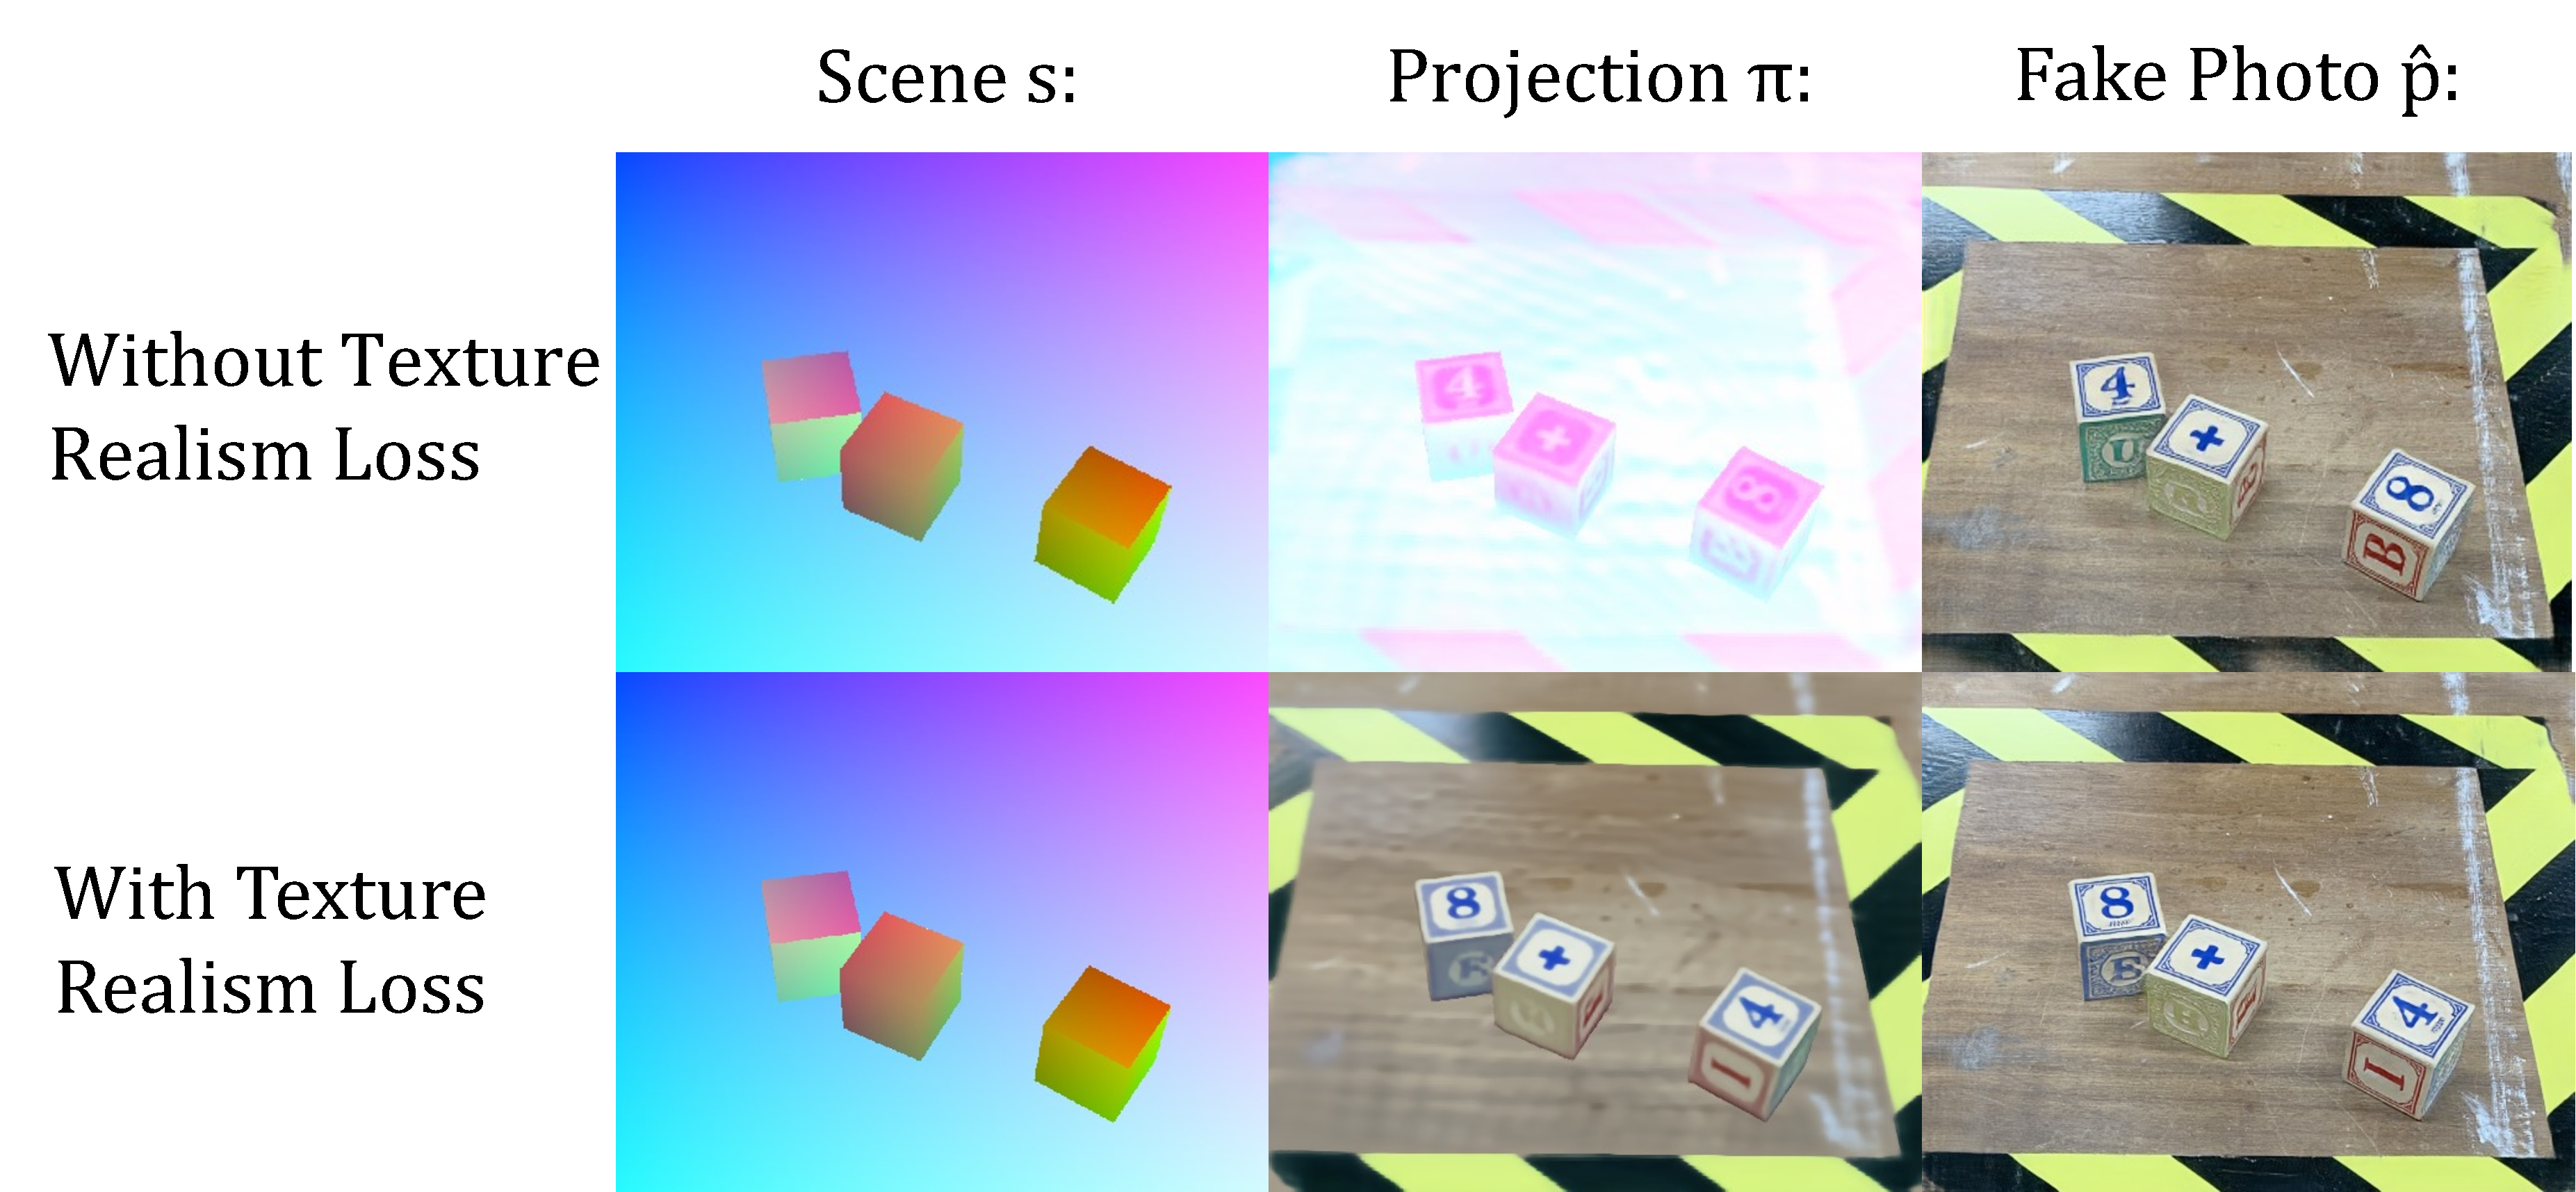
\includegraphics[width=1\linewidth]{../images/texture_realism_ablation.pdf}
% 			\vspace{-5pt}
            \vspace{-5pt}
			\caption{
				The neural texture looks more realistic with texture realism loss enabled. Note that the blocks show different letters because of different initializations and the symmetry of a cube - both solutions are valid texture assignments. 
			}
% 			\vspace{-10pt}
			\label{fig:texture_realism_ablation}
    \end{minipage}
    \vspace{-15pt}
\end{figure}
% \begin{figure}[thbp]
%     \vspace{-10pt}
% 	\begin{center}
% 		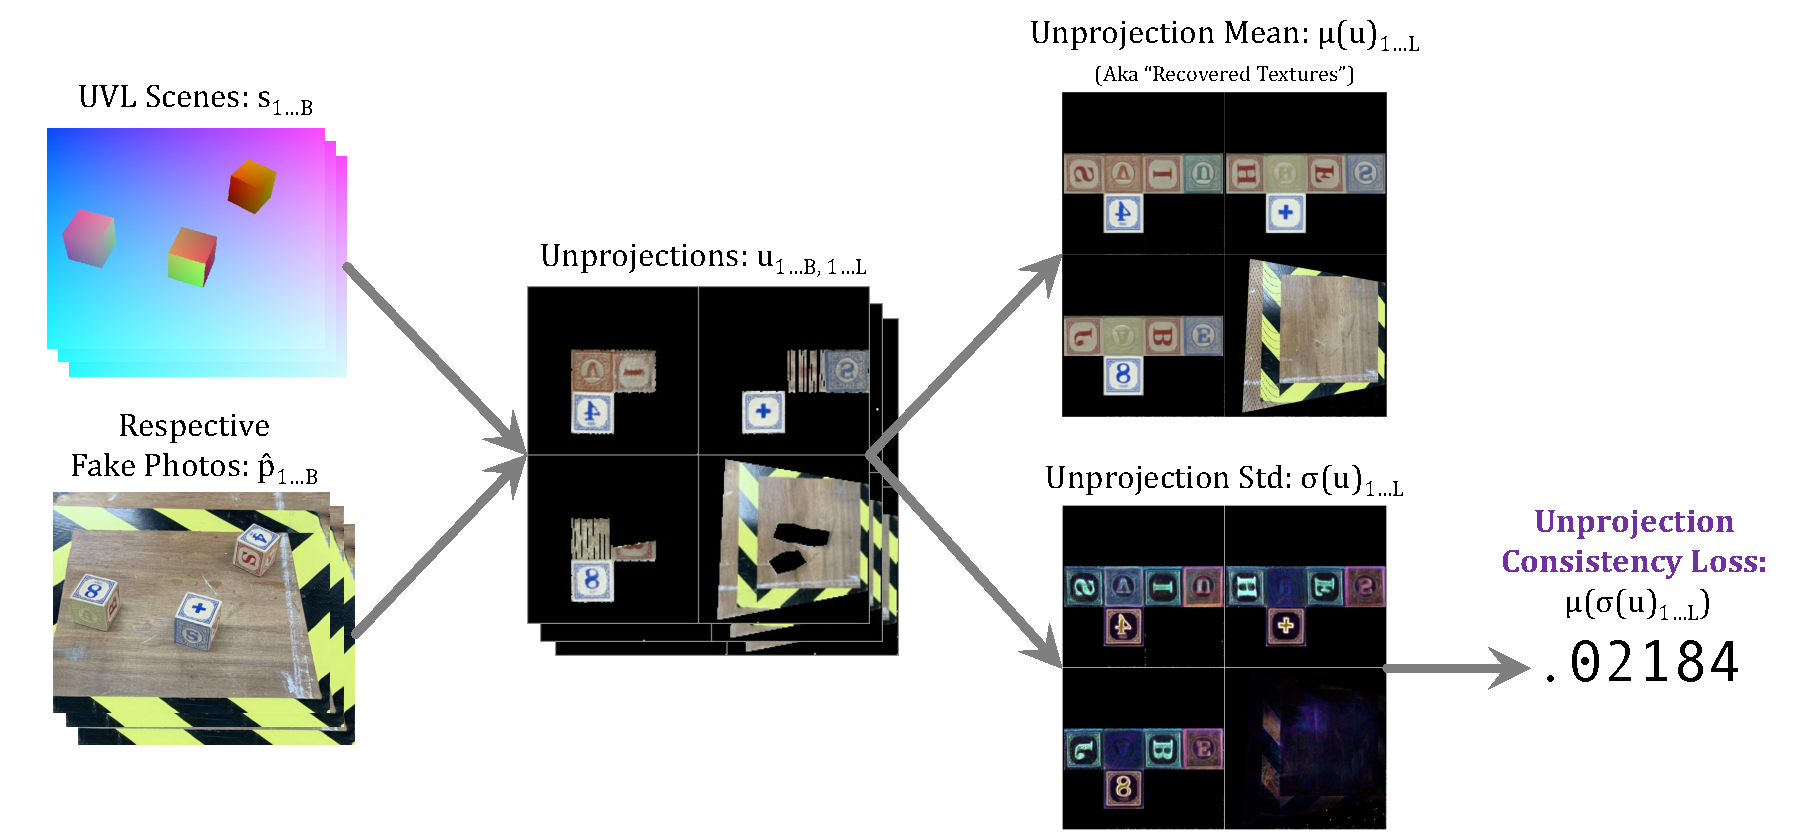
\includegraphics[width=.75\textwidth]{../images/unprojection_consistency_loss_without_reprojection.pdf}
% 	\end{center}
% 	\vspace{-5pt}
% 	\caption{
% 		This is the unprojection consistency loss used in Figure~\ref{fig:main_diagram}.
% 		The Unprojection Mean is not used in any losses, but help to illustrate the content in Section \ref{sec:texture_realism_loss}.
% 		% After calculating fake photos $\hat{p}_{1...B}$ from UVL scenes $s_{1...B}$ as seen in figure \ref{fig:main_diagram}, 
% 		% we can unproject fake photos $\hat{p}_{1...B}$ back into texture space to obtain $u_{1...B,\ 1...L}$ .
% 		% If the fake photos display consistent textures along their 3d surfaces, then the unprojected textures should be similar.
% 		% We can measure this similarity by taking the per-channel standard deviation of these unprojections, aka $\sigma(u)$, then averaging the result.
% 		% When the fake photos display similar surfaces, the unprojections will be similar making the unprojection consistency loss low.
% 		% Additionally, we can also calculate the average unprojection, which is useful for visualization purposes (it will look blurry if $\hat{p}$ is inconsistent).
% 	}
% 	\label{fig:unprojection_consistency_loss}
% \end{figure}
\vspace{-5pt}
\subsection{Unprojection Consistency Loss}
\vspace{-5pt}
	\label{sec:unprojection_consistency_loss}

		

		To keep the object surfaces consistent, we impose a pixel-wise ``unprojection consistency loss'' by unprojecting surfaces in fake photos back into the common texture space.
% 		\begin{equation}
% 			u\toNL=\text{unproject}(\ph\toN,s\toN)   \eqand  \lUC \Rightarrow u_1 \approx u_2 \dots \approx u_N
% 		\end{equation}
        Given a UVL scene $s$ and its respective fake photo $\ph$, the unprojection $\unprojection$ is obtained from assigning $(r,g,b)$ values at each pixel location $(x, y)$ of $\ph$ to its corresponding $(u, v, l)$ coordinates according to $s$. 
        % That is, we convert $s$ and $\ph$ to a key-value dictionary where the key is $(u,v,l)$ and the value is $(r,g,b)$, and such dictionary is $\unprojection$.
        For simplicity, we note
        \begin{equation}
            	\unprojection_{[u,v]}^{l}=\expectation\ph_{[x,y]} \quad s.t.~ (u,v,l) = s_{[x,y]},
        \end{equation}
        where the expectation $\mathbb{E}$ means we aggregate multiple $(r,g,b)$ vectors being assigned to the same $(u,v,l)$ coordinate by averaging them.
        In practice, $(u,v,l)$ are real numbers between $[0,1]$, where as each $\unprojection$ have to be rasterized, i.e., represented by $L$ images with a size of $(D\times D\times 3)$, where $L$ is the number of labels and $D\times D$ is the resolution of the unprojection. Therefore, we discretize and scale corresponding $(u,v,l)$ to integers so that each $(r,g,b)$ vector will be assigned to a pixel on $\unprojection$. For the exact implementation, please see our supplementary material.
        
        We obtain $N$ unprojections $\{\unprojection_{[u,v]}^{l,i}\}_{i=1}^{N}$ from a batch of $N$ UVL scenes and fake photos. The unprojection consistency loss is defined as the per pixel-channel standard deviation of $\unprojection$ over the batch
        \begin{equation}
            \ell_{UC} = \frac{1}{L\times D\times D\times 3}\sum_{l,u,v,c}\sigma(\{\unprojection^{l,i}_{[u,v,c]}\}_{i=1}^{N}),
        \end{equation}
        where $\sigma(\cdot)$ stands for the standard deviation function and $c \in \{1\dots 3\}$ is the channel index of $\unprojection$.
		%We sample a random batch of UVL scenes $S\toN$, and translate them into $\ph\toN$.
		%Using geometric knowledge of the scene encoded in $S\toN$, we individually unproject each $\ph^i \in \ph\toN$ back into texture space, to obtain $N$ sets of $L$ unprojected textures $u\toNL$.
		%We then use the per-pixel, batch-wise standard deviation of the unprojections as unprojection consistency loss $\lUC = \sigma(u\toNL)\toL$.
		%This loss observes how different these unprojections are from one another, and thus how different the object surfaces appear between translations. 
		We minimize $\lUC$ to encourage unprojections to be consistent across the batch. Intuitively, if $\lUC$ were $0$, it would mean the object surfaces in translations $\ph$ appear exactly the same in every scene. In addition, we call the mean of unprojections $\mu(\{\unprojection^{l,i}\}_{i=1}^N)$ as ``Recovered Textures'', visualzed in Figure~\ref{fig:first_diagram} and Section~\ref{fig:unprojection_consistency_loss}.

	%MOVE THIS TO APPENDIX
	% 	This loss is a fairly intuitive and effective way to maintain surface consistency. There are some caveats, howe/ver.
	% 	In order to produce a standard deviation greater than $0$, we must have a batch size greater than $1$.
	% 	Furthermore, environments that rarely show a particular region of a surface will rarely have $\lUC$ applied to that region because they're unlikely to show up twice in the same batch.
	% 	For this reason, $\lUC$ is most useful with large batch sizes.% because observing the same surface in multiple elements of a batch becomes more likely as the batch size increases. 
	% 	But because video memory limits our batch sizes, first-person environments might be more of a challenge for $\lUC$ - particularly when exploring multiple rooms (a task we haven't done though - should I mention this?)

		% To michael: Should we mention these caveats in this section, or mention them in the texture realism loss section? That section addresses all of these issues...
		
		% Also, you have to get lucky - two scene pictures have to show the same side of a cube for example. First person scenarios would be even worse.

		% %Unabbreviated
% 		\begin{equation}
% 			\unprojection_{c,U,V}^{n,i}=\expectation\ph_{c,x,y}^n 
% 			\eqand \bar{\unprojection}^i_{c,u,v}   =   
% 				\frac{1}{N} \lsum_{n=1}^N\unprojection^{n,i}_{c,u,v} 
% 			\eqand 
% 			\lUC=\frac{\lsum_{i=1}^L\lsum_{c=1}^3\lsum_{U=1}^{128}\lsum_{V=1}^{128}
% 			\sqrt[]{\frac{1}{N}\lsum_{n=1}^N\left(\bar{\unprojection}^i_{c,u,v}-\unprojection^{i,n}_{c,U,V}\right)^2}}
% 			{3\cdot128\cdot128\cdot L}
% 		\end{equation}
		
		%Abbreviated
		%To formally define $\lUC$ we define unprojections $\unprojection^{1...N,1...L}$ and mean unprojections (aka recovered textures) $\bar{\unprojection}^{1...L}$ 
		%with each $\unprojection^{n,i}\in\real^{3\times128\times128}$:
% 		\begin{equation}
% 			\unprojection_{U,V}^{n,i}=\expectation\ph_{x,y}^n 
% 			\eqand \bar{\unprojection}^i_{u,v}   =   
% 				\frac{1}{N} \lsum_n\unprojection^{n,i}_{u,v} 
% 			\eqand 
% 			%\lUC=\frac{\lsum_{i,U,V}
% 			%\sqrt[]{\frac{1}{N}\lsum_n\left(\bar{\unprojection}^i_{u,v}-\unprojection^{i,n}_{U,V}\right)^2}}
% 			%{128\cdot128\cdot L}
% 			\lUC=\mathbb{E}\left[
% 			\sqrt[]{\frac{1}{N}\lsum_n\left(\bar{\unprojection}^i_{u,v}-\unprojection^{i,n}_{U,V}\right)^2} \right]
% 		\end{equation}
% 		where $U=\lfloor128u\rfloor$ and $V=\lfloor128v\rfloor$ and $i=I(l)$ with
% 		%  $(u,v,l)=s^n_{1...3,x,y}$
% 		$u=s^n_{1,x,y}$, $v=s^n_{2,x,y}$, $l=s^n_{3,x,y}$
% 		for all 
% 		$n \in \{1...N\}$ , 
% 		$i \in \{1...L\}$ , 
% 		$x \in \{1...W\}$ , 
% 		$y \in \{1...H\}$ , 
% 		$U \in \{1...128\}$ , 
% 		$V \in \{1...128\}$.



	\subsection{Texture Realism Loss}
	\label{sec:texture_realism_loss}
        % \vspace{-7pt}
% 		\begin{figure}[thbp]
% 			\centering
% 				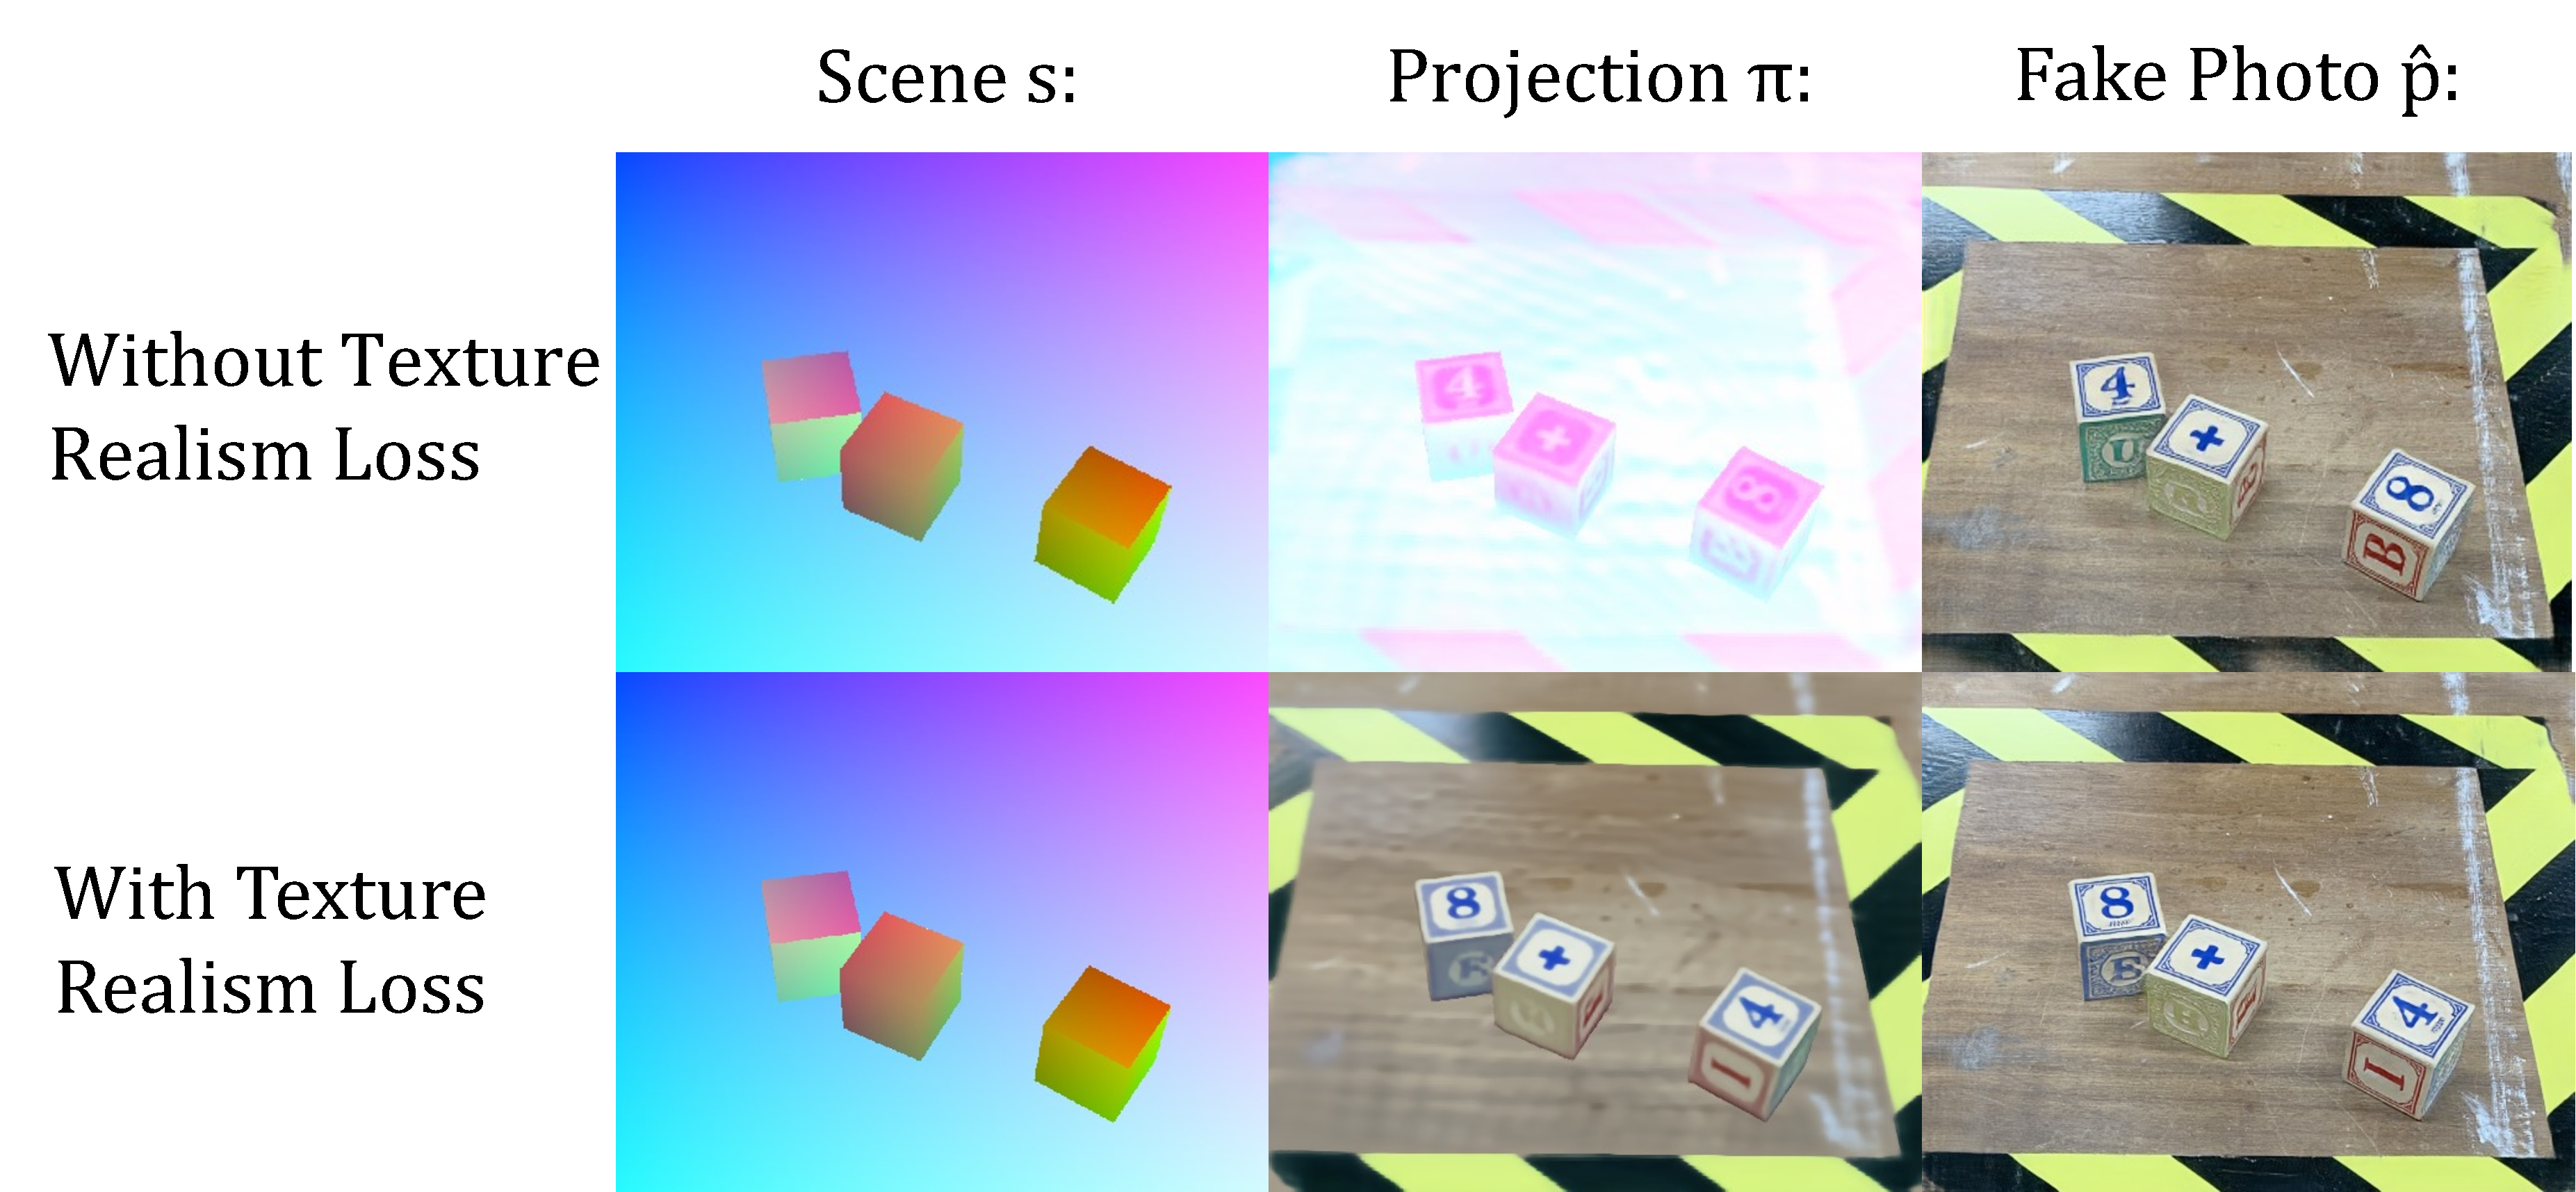
\includegraphics[width=0.5\textwidth]{../images/texture_realism_ablation.pdf}

% 			\vspace{-5pt}
% 			\caption{
% 				The neural texture looks more realistic with texture realism loss enabled. Note that the blocks show different letters because of different initializations and the symmetry of a cube - both solutions are valid texture assignments. 
% 			}
% 			\vspace{-10pt}
% 			\label{fig:texture_realism_ablation}
% 		\end{figure}



		To encourage the neural textures to look as realistic as possible, we try to make the projections look like the final output by introducing a ``texture realism'' loss $\lTR$. 
		$\lTR$ is an image similarity loss that makes $\pi$ look like its translation $\hat{p}$.
		% As it turns out, $\lTR$ is sufficiently powerful loss to generate surface-consistent translations even without $\lUC$, although the results are better when both losses are used.
		% This loss forces the neural textures to look realistic, instead of allowing them to have arbitrary colors.
		% In other words, $\lTR$ makes the neural textures more realistic by making their projections look more realistic, like the final outputs.
		\begin{equation}
			\lTR = \similar(\pi,\ph)
		\end{equation}
		% So far, we've taken an image translator $T$ and added neural textures $\psi$ and a surface consistency constraint $\lUC$. 
		% If we wanted to, could stop here - those formulations are sufficient to produce consistent sim-to-real translations.
		% However, we can improve this further.
		% Up until now we have not put any constraints on this neural texture. 
		Without $\lTR$, $\psi$ can look wildly different each time you train it.
		As seen in the top row of Figure \ref{fig:texture_realism_ablation}, the neural texture looks very unrealistic --- the colors are completely arbitrary.
% 		After adding $\lTR$ though, $\pih \approx \ph$ and thus the neural texture represents the textures of the objects in real life. 
        By adding texture realism loss $\lTR$, we make the textures $\psi$ more realistic. In practice, this makes TRITON less likely to mismatch the identity of translated objects.
		% The image similarity loss used in $\lTR$ is calculated the same way image similarity losses are calculated in section \ref{sec:image_translation}: L2 loss minus MSSSIM.
		%As it turns out, we can achieve surface-consistent translations just using $\lTR$, without $\lUC$.
		%The the reverse is also true: $\lTR$ is sufficient to ensure surface consistency without $\lUC$.
		%Using both, however, yields better results than either loss alone. \\
		% For an explanation of why this is the case, see the appendix \ref{sec:texture_realism_theory}.
		%With that said, there are some advantages to using $\lTR$ alone: when just using $\lTR$ you can use batch sizes as small as $N=1$, allowing you to save video memory. 
		%Using $\lTR$ is also more numerically stable, as you no longer have to worry about whether the same surfaces are seen across multiple scenes in a batch as you would with $\lUC$.

		% We introduce a new loss, called texture realism loss that fixes this: $\lTR$ is an image similarity loss that encourages $\pi \approx \ph$.
		% This loss forces the neural texture to approximate the albedo of the surfaces in a scene.

		% These images could be regularized so that they're the same every time.
		% 
		% To do this we put a penalty on the latent texture that makes it $\pi$ look like its translation $\hat{p}$. 
		% 
		% We use l2 and msssim losses to do this.
		% 
		% This helps improve the translations.
		% 
		% There are some advantages over unprojection consistency though: 
		% smaller batch sizes (even a batch size of 1, which UC cant do),
		% you don't have to get lucky (the more chaotic, or even the more zoomed in a dataset becomes the less likely there is to be any collisions)

	%===============================================================================
\vspace{-8pt}
\section{Experiments}\label{sec:results}
\vspace{-3pt}
\subsection{Datasets}
\label{sec:datasetsresults}
\vspace{-2pt}
%Here we detail the datasets used in our experiments.
% We constructed multiple datasets for our experiments.
We constructed two datasets AlphabetCube-3 and RobotPose-xArm to benchmark different image translators in many perspectives.
In our setting, each dataset is composed of two sets of unpaired images: UVL scenes from a simulator and real photographs.
Note that the images in all datasets are unpaired and UVL scenes only rely on rough 3d models of the objects in the scene without need of precisely aligning objects in the simulator to the real world.
% . They are all unpaired, and have RGB values ranging from 0 to 1.
We use AlphabetCube-3 for image translation quality evaluation, and RobotPose-xArm for sim2real policy learning evaluation.

% The first dataset we particularly use for the offline evaluation is the three-block dataset.  


% [[Insert photographs and UVL maps here; a digram showing each dataset we describe here and 1 or two samples of each domain in each dataset]]

% In this paper, we'll mostly focus on a hand-collected dataset that involves three alphabet blocks that are moved across a table.
% Alphabet blocks were chosen because they all have the same geometry (a cube), but have very distinct semantic textures that will make temporal inconsistency obvious to the human eye.
% This dataset is analogous to data that would be collected for a third-person robotic grasping task.
% However, other objects (such as cans of soda, apples, cloves of garlic, etc) are also for generating other results in this paper. ((TODO: Detail the five object tests and five cube tests and other stuff like shiny cans etc)).

% There are two components to this dataset: Simulated data in the form of UVL scenes, and photographs.
% The camera in the simulation is positioned in approximately the same place as the real camera, with approximately the same field of view.
% In both domains of this dataset, the camera never moves. Instead, the objects are randomly positioned and rotated on the table.
% In both the simulation and in real life, these objects are randomly translated along the x and y-axis of the table, as well as rotated on the z-axis.

% There are 200 photographs in this dataset, and they are recorded as RGB jpg images.
% There are 3000 synthetic images in this dataset, in the form of UVL images.
% These UVL images are also encoded as RGB images, but provide information about the geometry of a scene.
% UVL images are composed of both a UV map and a label map and are summarized in figure \ref{fig:uvl_explanation}.
% To avoid positional rounding errors, UVL images are encoded as EXR files: an image format that supports floating-point values.

% The pixels in a UVL image are visualizable in RGB space because, like RGB images, each pixel is a vector with 3 values. The first two channels, U and V, are floating point values between 0 and 1. The L channel is also a floating point value between 0 and 1, it has a second meaning. There are only a finite number of label values (corresponding to the number of learnable textures). The rank of a particular L value is used to index these textures.

% In the three-cube dataset we have 4 textures, and UVL scenes contain label values $l \in [\frac{0}{3}, \frac{1}{3},\frac{2}{3}, \frac{3}{3}]$. A pixel in a UVL scene $l=\frac{2}{3}$ will get indexed to the third texture, because $\frac{2}{3}$ is the third smallest label value.

% %===============================================================================

% Domain A and B
% p hat
% s hat

%\subsection{Qualitative Evaluation Results}
%We show qualitative evaluation results ....[TODO]
\begin{figure}[th]
	\begin{center}
		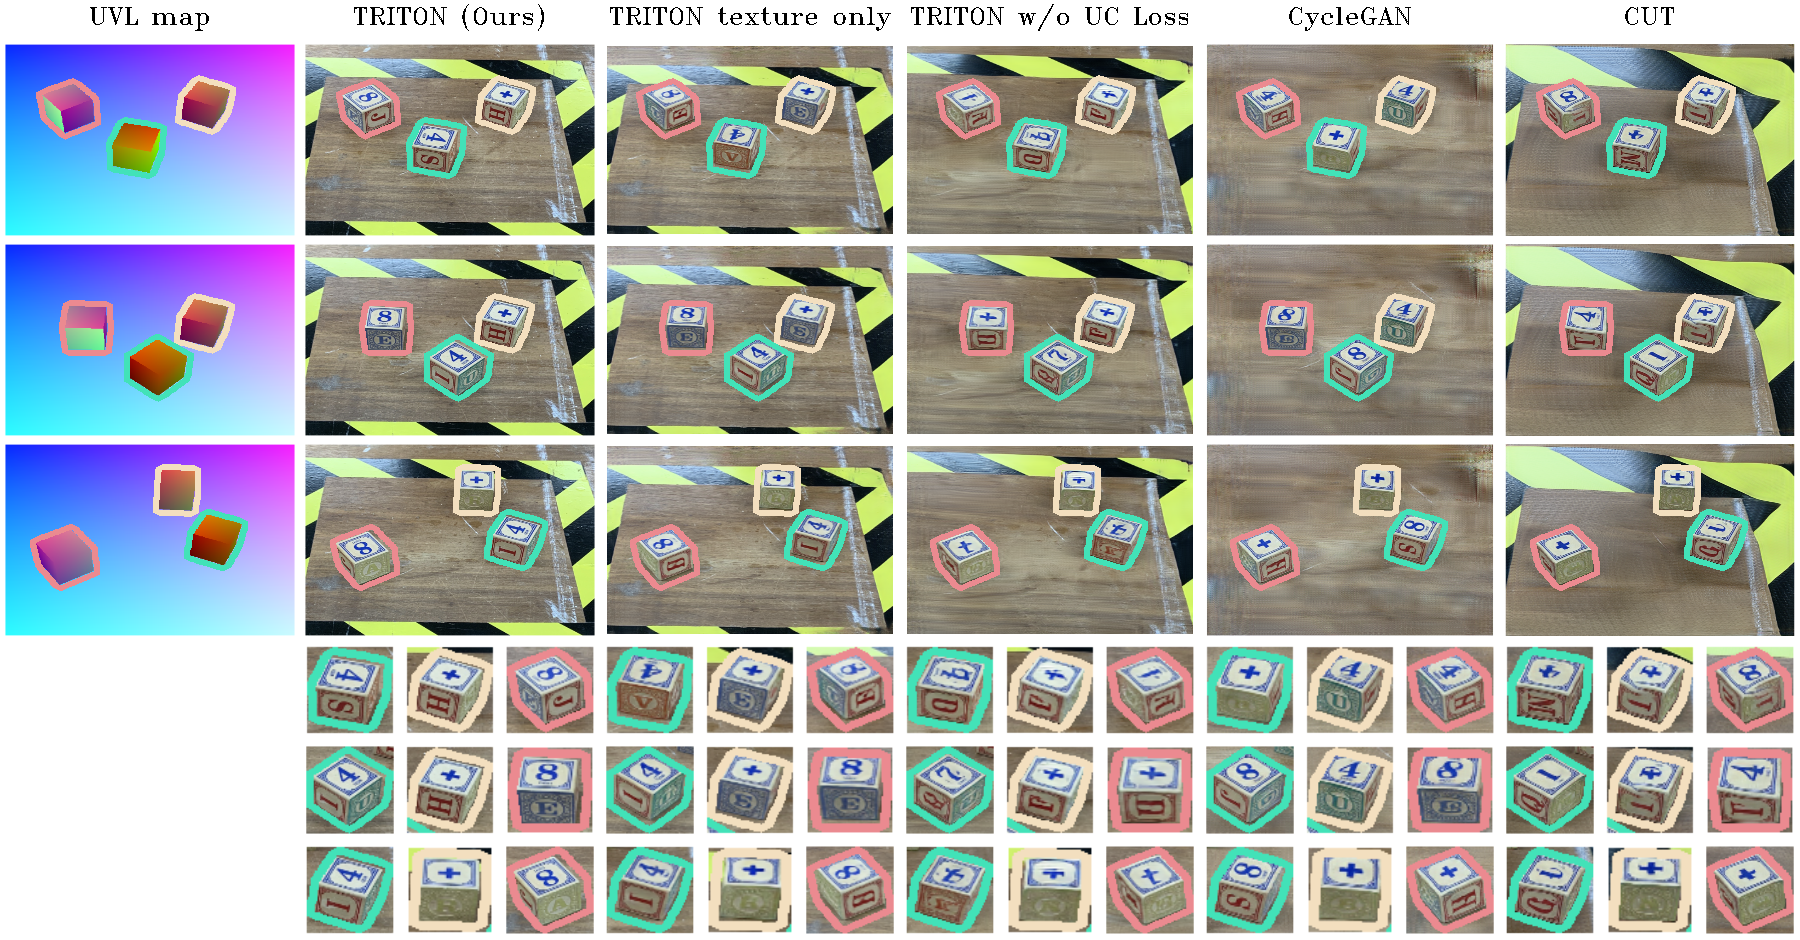
\includegraphics[width=.9\textwidth]{../images/frame_inconsistency_diagram.png}
	\end{center}
	\vspace{-7pt}
	% Each outline color corresponds to the same cube.
	% The same cubes are marked with the same colored outlines across all photos.
	% For the same cube, we expect to see the same number on the top of the cube regardless of its placement.
	\caption{
	    Comparison of image translation methods.
	    The first column is the UVL map as the input.
	    The other columns are results using different image translation methods.
		Each row of images shows a different random placement of objects in the scene.
		TRITON consistently outputs high quality results over different object arrangements. 
		``TRITON Texture-Only'' stands for TRITON without two surface consistency losses $\lUC$ and $\lTR$.
		% Each column of images is a different image translation algorithm.
		% The same cube is marked with the same color outline across all photos.
		% TRITON is consistent: for example, the cube outlined as yellow always has an 8 on the top.
		% Meanwhile, CycleGAN for example shows a 4 on the top of that cube in the top two rows, but an 8 and a 7 in the next two rows.
		% Because of the symmetry of the cubes, and the unsupervised training, it is arbitrary which synthetic cube gets which symbol after training - but whatever it chooses, it should be consistent between placements.
		% CUT and CycleGAN are not consistent, while TRITON is.
		% TODO: Update the images in this to have the latest training iteration...
		}
		\vspace{-15pt}
		\label{fig:frame_inconsistency_diagram}
	\end{figure}
	

    % \begin{figure}[thbp]
    % 	\begin{center}
    % 		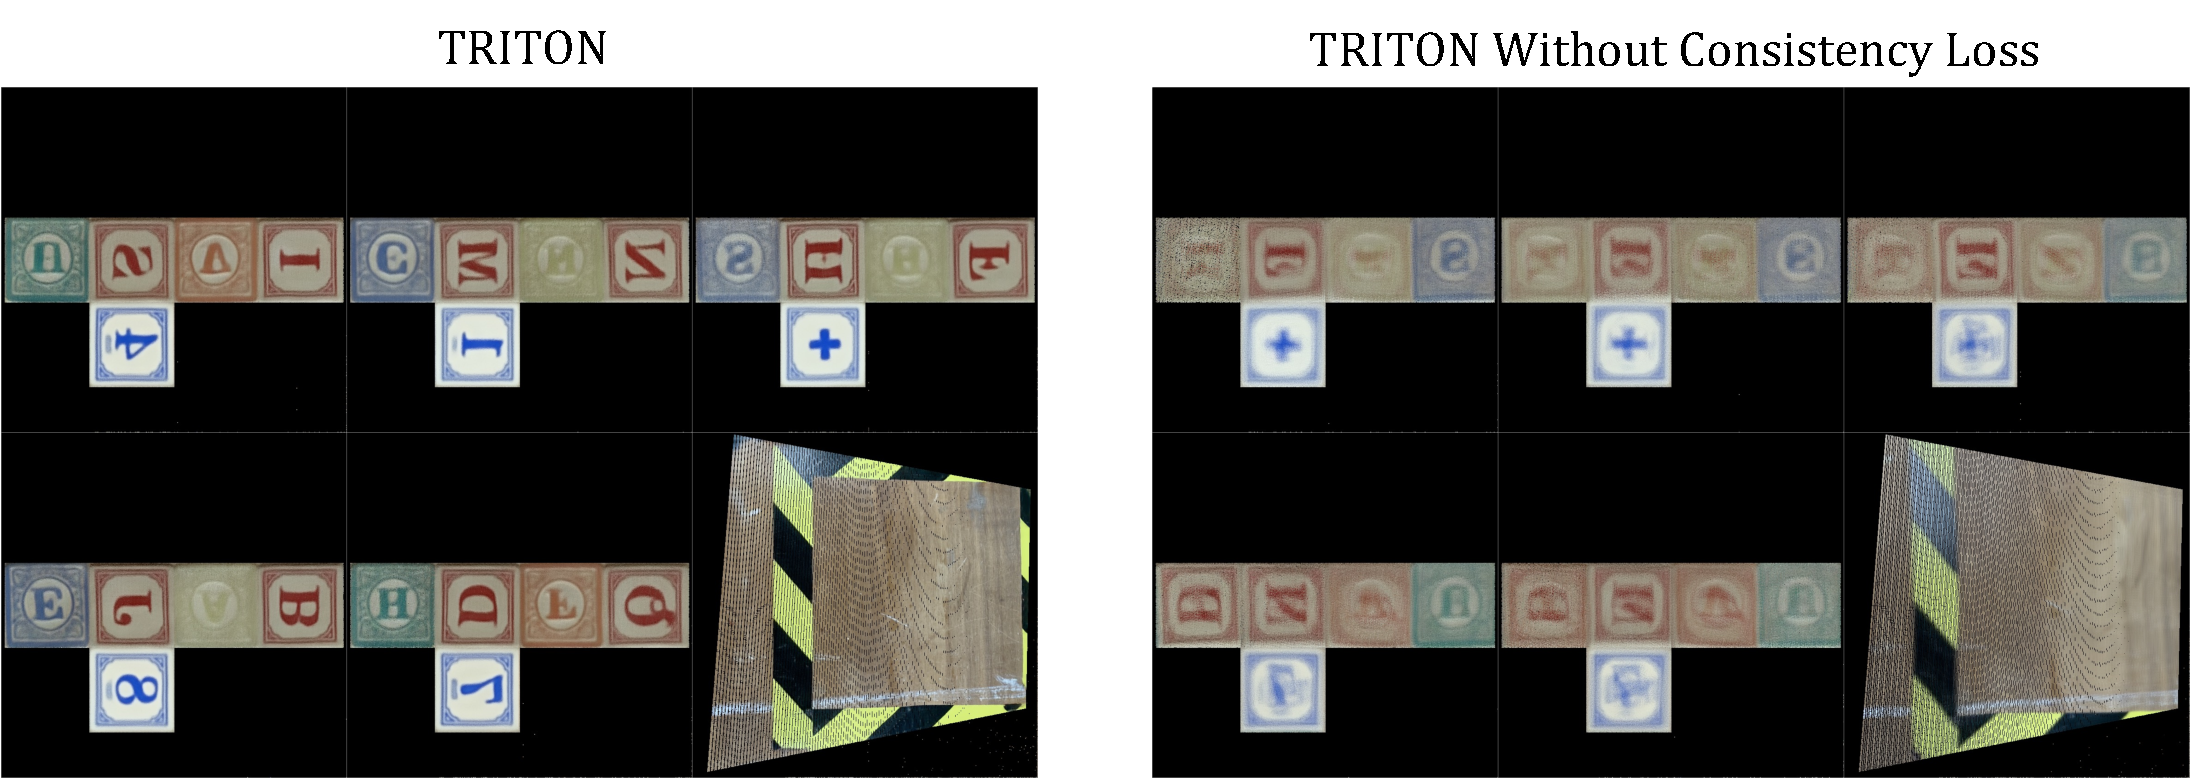
\includegraphics[width=\textwidth]{../images/blurry_recovery.pdf}
    % 	\end{center}
    % 	\caption{
    % 		The recovered texture is more crisp when we have surface consistency losses $\lUC$ and $\lTR$ enabled.
    % 		[[TODO: include cyclegan and other algorithms here]]
    % 	}
    % 	\label{fig:blurry_recovery}
    % \end{figure}
	% 	Alphabet Three							
	% 	Masked				Unmasked			
	% 	LPIPS		L2		LPIPS		L2	
	% 	Sync	Unsync	Sync	Unsync	Sync	Unsync	Sync	Unsync
	% Pure MUNIT	0.0437	0.0373	0.00500	0.00490	0.434	0.402	0.0425	0.0392
	% Texture Only	0.0442	0.0386	0.00586	0.00589	0.285	0.255	0.0364	0.0310
	% Texture Reality	0.0286	0.0267	0.00479	0.00478	0.117	0.1157	0.0123	0.0122
	% CycleGAN			TODO: Sync with respect to L2, so sync is always ≥ unsync					
	% CUT				TODO: Google Synthetic Dataset				

	 
% \subsection{TRITON evaluation}
% \vspace{-1pt}
\subsection{Image Translation Evaluation on AlphabetCube-3}
% \vspace{-3pt}
AlphabetCube-3 dataset features a table with three different alphabet blocks on the top.
% All blocks are randomly translated along the X and Y axes and rotated randomly along the Z axis.
The dataset contains 300 real photos and 2000 UVL scenes from a simulator.  
Each photograph features these three cubes with a random position and rotation.
In this section, we evaluate the image translation accuracy of the TRITON and other image translation methods using AlphabetCube-3.

Figure~\ref{fig:frame_inconsistency_diagram} shows qualitative results on the dataset.
% The first column is the input UVL map for all the image translators and other columns are the results.
% ``TRITON texture only'' stands for TRITON without two view consistency losses $\lUC$ and $\lTR$.
% Each row of images shows a different random placement of objects in the scene except for the last row where we collect all the translated cubes from different scenes.
% We use contours in different colors to help identify three cubes.
From Figure~\ref{fig:frame_inconsistency_diagram} we find that TRITON consistently outputs high quality results over different object arrangements.
The textures keep aligned even when the position of blocks change dramatically over multiple scenes (See examples in green rectangle in Figure~\ref{fig:frame_inconsistency_diagram}).
In contrast, though MUNIT~\cite{munit} and CycleGAN~\cite{cyclegan} manage to generate realistic images, the surfaces of the cubes are either consistent over scenes (See exsamples in the red rectangle) or replicated by mistake (See examples in the orange rectangle).
Also note that the floor background of the outputs from CycleGAN are quite different from the ground truth.
CUT~\cite{cut} fails to generate meaningful images regarding both the foreground blocks and the background.

We further conduct quantitative experiments and the results are shown as Table~\ref{tab:quantitative}.
In this evaluation we manually align the simulator with 14 photos of different real world scenes and generate the UVL maps for translation.
We measured the LPIPS~\cite{lpips} and $l2$-norm between the translated images and the real images using multiple configurations.
`Masked' means we mask out the background (which is the floor in AlphabetCube-3 dataset) and only measure the translation quality w.r.t three foreground blocks.
For the `unmasked' tests, we compare the whole image without any masking instead, and the background contributes much more to the losses due to its larger area.
Similar to the qualitative results, TRITON consistently outperforms other methods under different metrics and configurations.
Further ablations TRITON w/o $\psi, \lUC, \lTR$ and TRITON w/o $\lUC, \lTR$ show the importance of the new losses we introduce.



\begin{comment}
Comment from Xiang: it might be better to have a short introduction on training details if we have space.
\end{comment}



% ... shows ...

	%CREATED WITH https://www.tablesgenerator.com/# -- this website is wonderful!!
\begin{comment}
\begin{table}[thbp]
    \caption{Ground truth comparison evaluations for TRITON. Masked and Unmasked mean xxxxxx. Sync and Unsync mean xxxxx. L2 is xxxx LPIPS is xxxxxx. TRITON is xxxxxxx. }
    \label{tab:quantitative}
	\resizebox{\textwidth}{!}{
        \begin{tabular}{lcccccccc}
        \toprule
        & \multicolumn{4}{c}{Masked} & \multicolumn{4}{c}{Unmasked}  \\
        \cmidrule(lr){2-5} \cmidrule(lr){6-9} & \multicolumn{2}{c}{LPIPS ($\times 10^{-1}$) $\downarrow$} & \multicolumn{2}{c}{L2 ($\times 10^{-2}$) $\downarrow$}  & \multicolumn{2}{c}{LPIPS ($\times 10^{-1}$) $\downarrow$}  & \multicolumn{2}{c}{L2 ($\times 10^{-2}$) $\downarrow$}   \\
        \cmidrule(lr){2-3} \cmidrule(lr){4-5} \cmidrule(lr){6-7} \cmidrule(lr){8-9}
        Algorithm  & Sync    & Unsync   & Sync      & Unsync    & Sync   & Unsync  & Sync     & Unsync \\
        \midrule
        CycleGAN & 0.450 & 0.379 &  0.559 &  0.554 &  6.02 &  5.93 &  4.25 &  4.23 \\
        CUT                           & 0.469                        & 0.382                        & 0.553                        & 0.526                        & 5.40                        & 5.34                        & 6.37                        & 6.29\\
        \midrule
        TRITON w/o $\psi, \lUC, \lTR$ & 0.437                        & 0.373                        & 0.500                        & 0.490                        & 4.34                        & 4.02                        & 4.25                        & 3.92                        \\
        TRITON w/o $\lUC, \lTR$       & 0.442                        & 0.386                        & 0.586                        & 0.589                        & 2.85                        & 2.55                        & 3.64                        & 3.10                        \\
        \textbf{TRITON}                        & \textbf{0.286}               & \textbf{0.267}               & \textbf{0.479}               & \textbf{0.478}               & \textbf{1.17}               & \textbf{1.16}              & \textbf{1.23}               & \textbf{1.22}               \\
        \bottomrule
        \end{tabular}
	}
\end{table}
\end{comment}

\begin{table}[thbp]
    \centering
    \setlength{\tabcolsep}{2pt}
    \caption{Quantitative results on AlphabetCube-3. LPIPS~\cite{lpips} and $l2$-norm between the translated images and the real images are reported. We exclude backgrounds in the `Masked' configuration. TRITON consistently outperforms other methods in different metrics and configurations}
    \label{tab:quantitative}
\resizebox{.80\textwidth}{!}{
        \begin{tabular}{lcccc}
        \toprule
        & \multicolumn{2}{c}{Masked} & \multicolumn{2}{c}{Unmasked}  \\
        \cmidrule(lr){2-3} \cmidrule(lr){4-5} & LPIPS ($\times 10^{-1}$) $\downarrow$ & L2 ($\times 10^{-2}$) $\downarrow$  & LPIPS ($\times 10^{-1}$) $\downarrow$  & L2 ($\times 10^{-2}$) $\downarrow$   \\
        \midrule
        CycleGAN & 0.450 &   0.559 &    6.02 &    4.25  \\
        CUT & 0.469 & 0.553  & 5.40  & 6.37 \\
        \midrule
        TRITON w/o $\psi, \lUC, \lTR$ & 0.437   & 0.500  & 4.34  & 4.25  \\
        TRITON w/o $\lUC, \lTR$       & 0.442  & 0.586  & 2.85 & 3.64 \\
        \textbf{TRITON} & \textbf{0.286}  & \textbf{0.479}  & \textbf{1.17}  & \textbf{1.23} \\
        \bottomrule
        \end{tabular}
	}
\end{table}

% [[Figures: Show these results and explain why we have a mask on some of them]]

% TODO: Explain what sync and unsync mean, retrieve the results for CycleGAN and CUT
\vspace{-5pt}
\subsection{Sim2real Transfer for Robot Learning}
\begin{figure}[thbp]
    \centering
    \vspace{-10pt}
    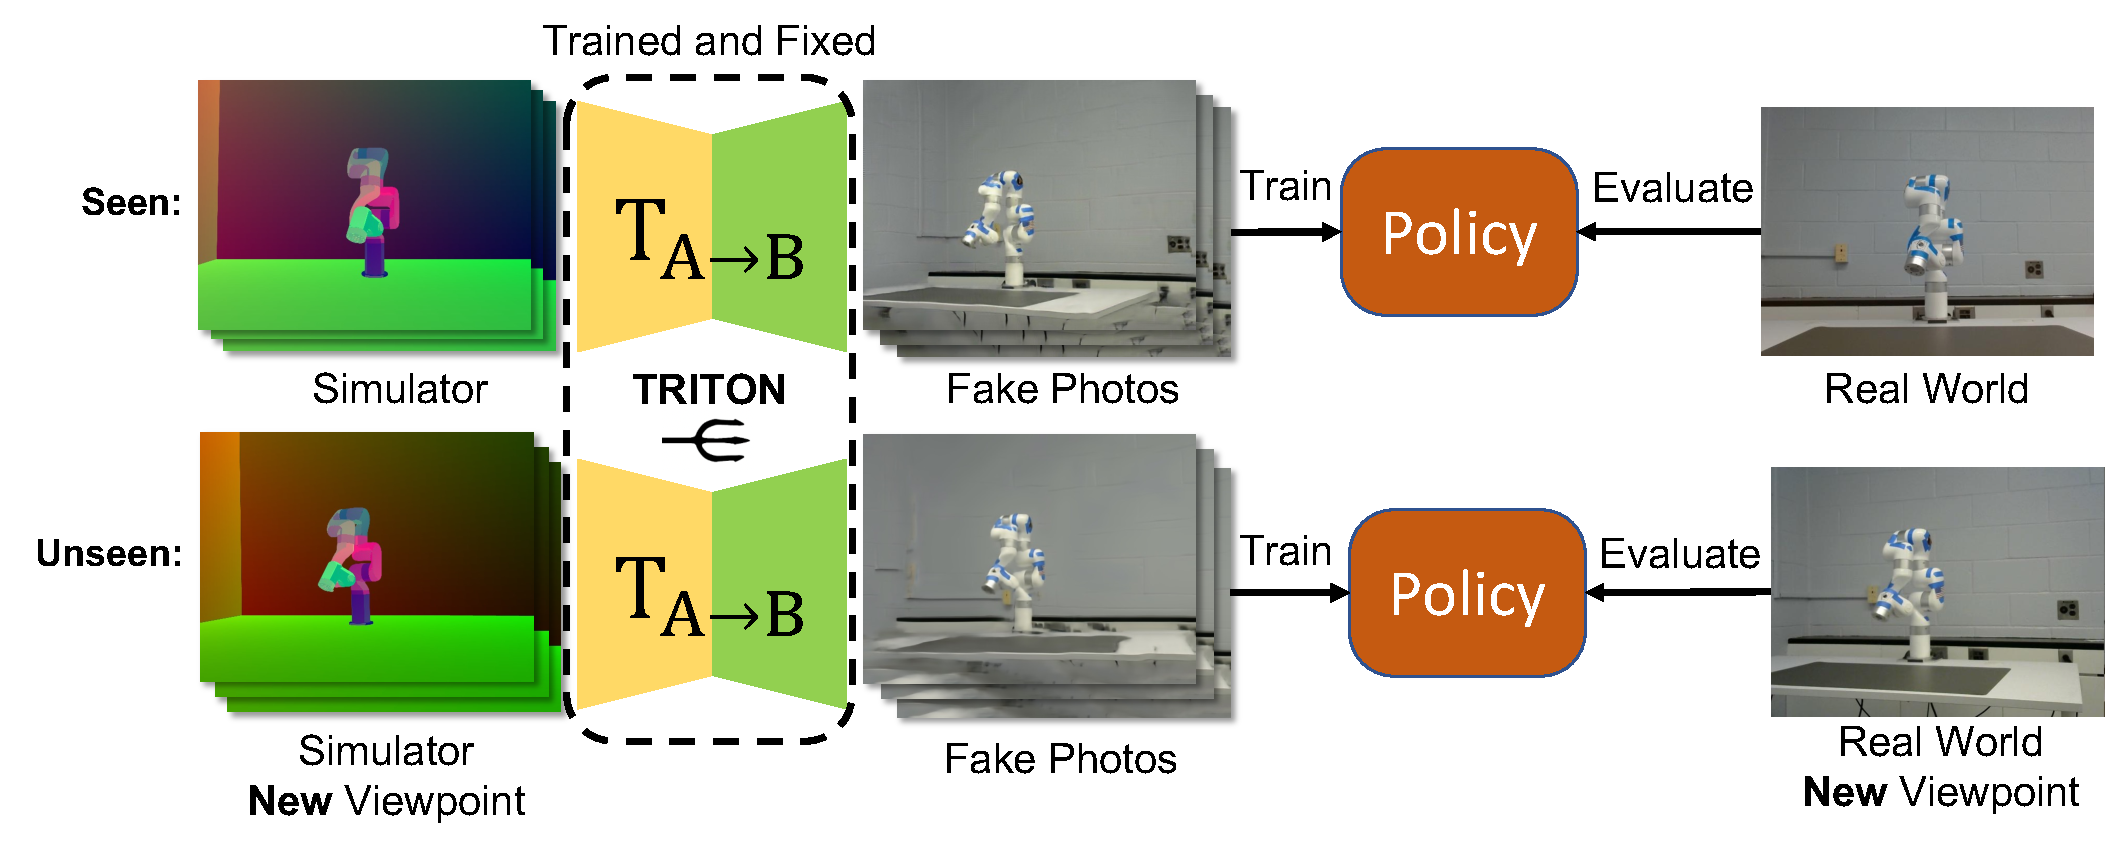
\includegraphics[width=.8\textwidth]{../images/sim2real_framework.pdf}
    \vspace{-10pt}
    \caption{Sim2real framework of using TRITON. We evaluate in two settings: Seen and Unseen. In Unseen, we use a new camera viewpoint to train and evaluate the policy. This new viewpoint is not used for training TRITON. }
    \vspace{-5pt}
    \label{fig:sim2realframework}
\end{figure}
In this section we demonstrate how TRITON improves sim2real transfer for robot policy learning. To this end, we first train TRITON on a dataset consist of unpaired UVL scenes from a robot simulator (Gazebo) and photos from the real robot. Once TRITON is trained, we learn the robot policy while only utilizing the simulator. The input of the policy is the fake photo $\ph$ translated from the simulated UVL scene using TRITON's translator $T_{A\to B}$. Finally, the trained policy is directly evaluated on the real robot, taking real photos $p$ as input.

Ideally, a good image translation model makes $\ph$ similar to $p$, so that the policy trained on synthesized photos will transfer to real domain seamlessly and will have better performance. All our policies are learned with zero real-world robot interaction with the environment.

\textbf{Task} We use a robot pose imitation task for our experiments. Given the input of a photo of real robot pose, the policy outputs robot controls to replicate that target pose. We measure the angular error between the replicated and target poses as our evaluation metric:$\sqrt{\sum_{j} (\hat{a}_j - a_j)^2}$,
where $\hat{a}_j$ and $a_j$ are replicated and target joint angles respectively, and $j$ is the joint index. We use an xArm robot which has seven joints. We also attached patterns and tapes on the robot to make its texture more challenging to model.

\textbf{Robot policy and Baselines}
Since the sim2real formulation allows benefiting from abundant training data using the simulator, we use behavior cloning to train a good robot policy.
The policy is implemented with a CNN~\cite{dqn}.
We compare TRITON against two baseline image translation methods: CycleGAN~\cite{cyclegan} and CUT~\cite{cut}, by replacing TRITON with each baseline method respectively in the above pipeline. The robot policy learning method is same for all the methods.

\textbf{Evaluation Settings} We introduce two main evaluation settings, \textbf{Seen} and \textbf{Unseen}. In the \textbf{Seen} setting, the policy is trained and tested using the same camera viewpoint that is used during TRITON (or a baseline translator) training. Whereas in \textbf{Unseen} setting, we introduce a camera at a new viewpoint for training and testing the policy. That is, the image translator has to generate the fake photos out of its training distribution (seen camera viewpoints), which becomes a challenging task for the translator. We also vary input image resolutions to show the power of photo-realistic images in higher resolutions.

\begin{figure}[tbhp]
    \centering
    \vspace{-3pt}
    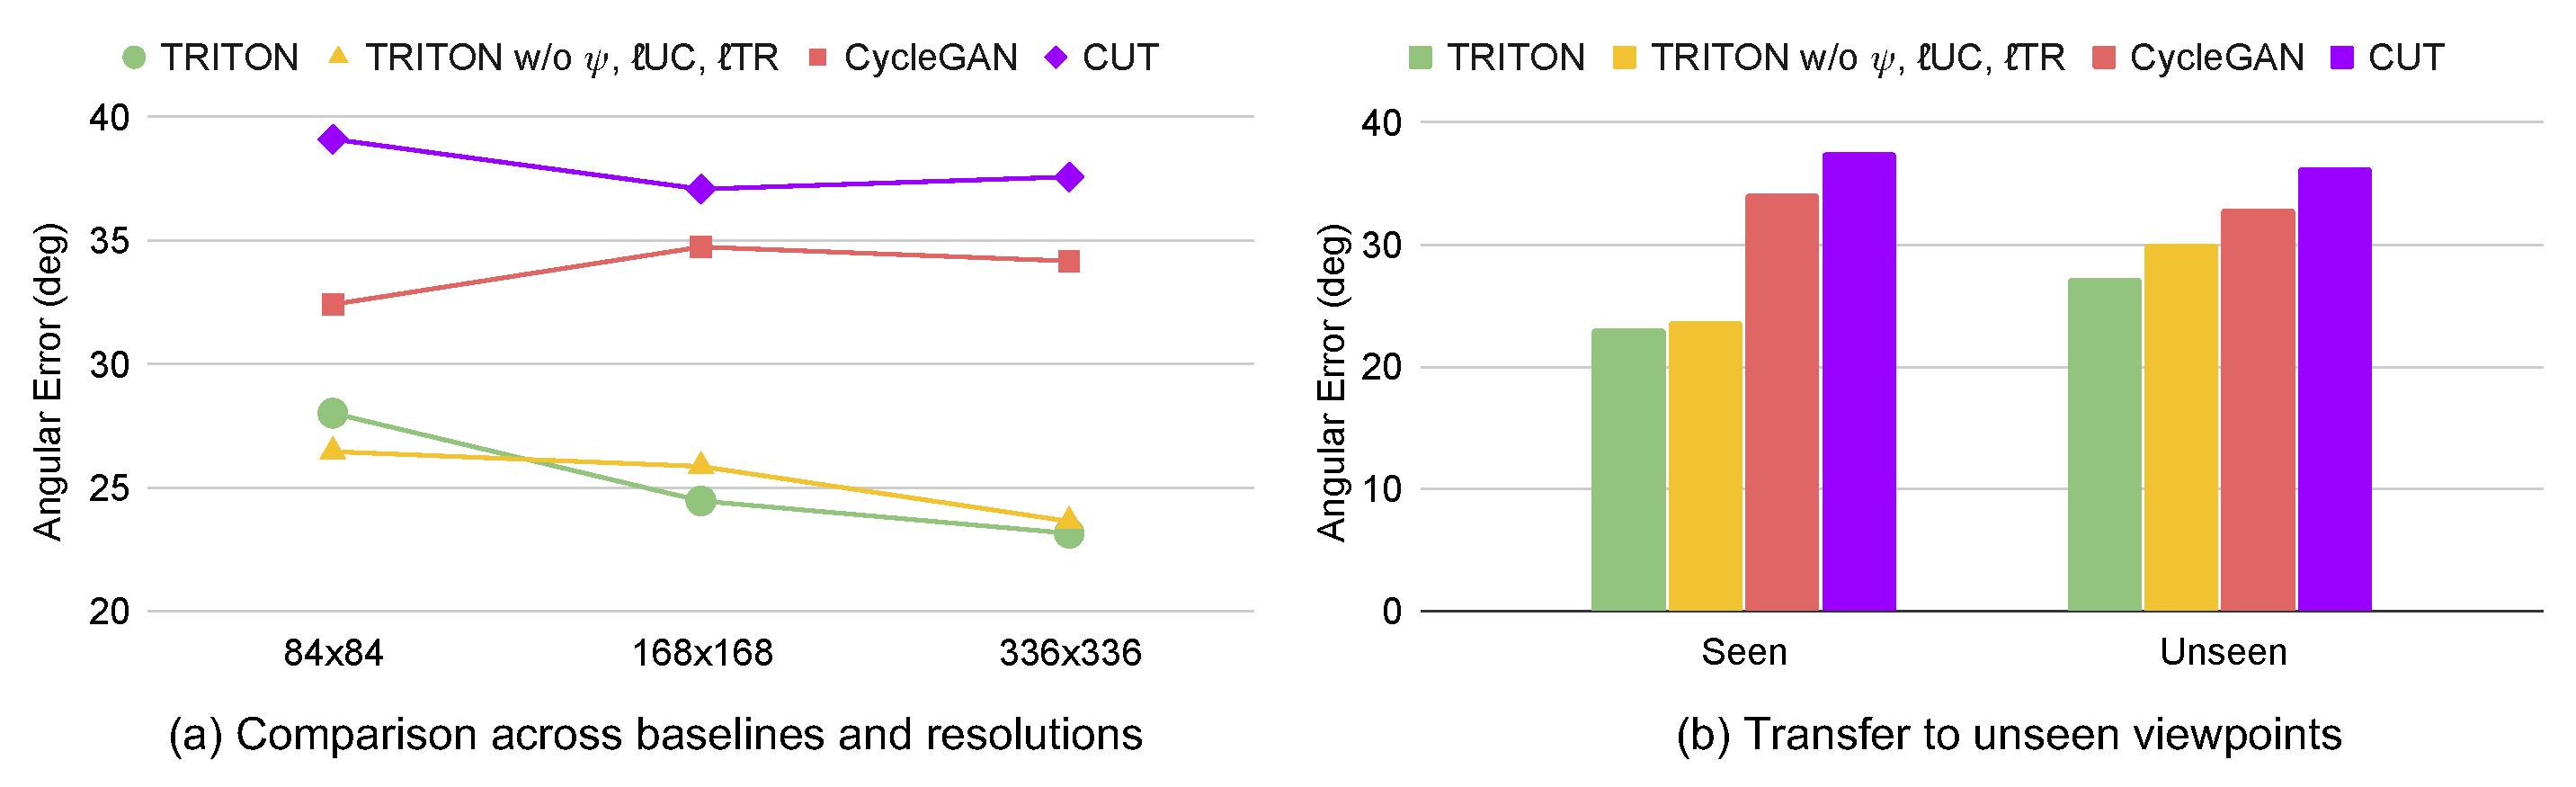
\includegraphics[width=.95\textwidth]{../images/sim2real_res.pdf}
    \vspace{-5pt}
    \caption{Evaluation results of sim2real robot learning. We compare TRITON against two baselines and one TRITON variant w/o $\psi,\ell_{UC},\lTR$ across 3 different input image resolutions. TRITON outperforms CycleGAN~\cite{cyclegan} and CUT~\cite{cut} consistently across (a) all resolutions and (b) unseen viewpoints. Results in (a) are from Seen setting only. Results in (b) are from 336x336 resolution. }
    \label{fig:sim2real}
    \vspace{-3pt}
\end{figure}

\textbf{Results} Figure~\ref{fig:sim2real} shows the evaluation results of the sim2real transfer. Both Seen and Unseen evaluations show that TRITON outperforms baselines consistently. In Figure~\ref{fig:sim2real}(a), we find that TRITON continuously improves from low to high resolutions due to its ability to generate more photo-realistic images compared to the baselines.
%This is because in low resolution (eg. $84\times 84$), the details in images are not important, whereas in high resolution ($336\times 336$), artifacts from imperfect translator are clearer and may harm policy learning.
From Figure~\ref{fig:sim2real}(b), we confirm that TRITON outperforms the others also in the Unseen setting, showing that TRITON learns image translations that are generalizable to new viewpoints while others are limited.
In the comparison against TRITON w/o $\psi,\ell_{UC},\lTR$, TRITON outperforms this variant consistently except the lowest resolution. This again shows the effectiveness of $\psi$, $\ell_{UC}$ and $\lTR$ to generate photo-realistic images, and such high quality images are important in higher resolutions for sim2real transfer.






%===============================================================================
\vspace{-8pt}
\section{Limitaions}
\label{sec:Limitations} 
% There are limitations of TRITON. 
TRITON relies on 3D models of objects in order to generate photo-realistic images, making it less applicable when the geometry of an environment is unknown. Acquiring such 3D models could be challenging in the wild, especially in robots allowed to roam the world. TRITON is not able to handle transparent objects, because the UVL format is opaque. Moreover, the probability of incorrectly matching textures to objects increases as the number of object classes increases.

\acknowledgments{We thank Srijan Das and Kanchana Ranasinghe for valuable discussions. This work was supported by the National Science Foundation (IIS-2104404 and CNS-2104416).}
%===============================================================================

% \section{Citations} 
% \label{sec:citations} 

% Citations can be made using either \textbackslash citep\{\} or \textbackslash citet\{\}, depending on the appropriateness. To avoid the citation moving to the next line, it is often a good practice to replace the space before with a tilde (\~{}) character.
% Example 1: ``CoRL is the best conference ever~\citep{fourier_feature_networks}.''
% Example 2: ``\citet{fourier_feature_networks} proved, both theoretically and numerically, that CoRL is the best conference ever.''

%===============================================================================

% \clearpage
% The acknowledgments are automatically included only in the final and preprint versions of the paper.


%===============================================================================

\bibliography{example}  % .bib

% \clearpage

\section{Appendix} 

\subsection{Neural Neural Textures: More Details}

	In section \ref{sec:neural_tex}, we mentioned that neural neural textures learn better than raster neural textures. 
	TRITON can be ablated to use raster textures. Let's call this version ``Raster TRITON''. 
	Raster TRITON is extremely sensitive to the resolution of its neural texture, and can be numerically unstable if that resolution is too high.
	In comparison, regular TRITON's neural neural textures don't have a specific resolution: they are continuously defined over the UV domain using Fourier feature networks.

	\begin{figure}[H]
		\begin{center}
			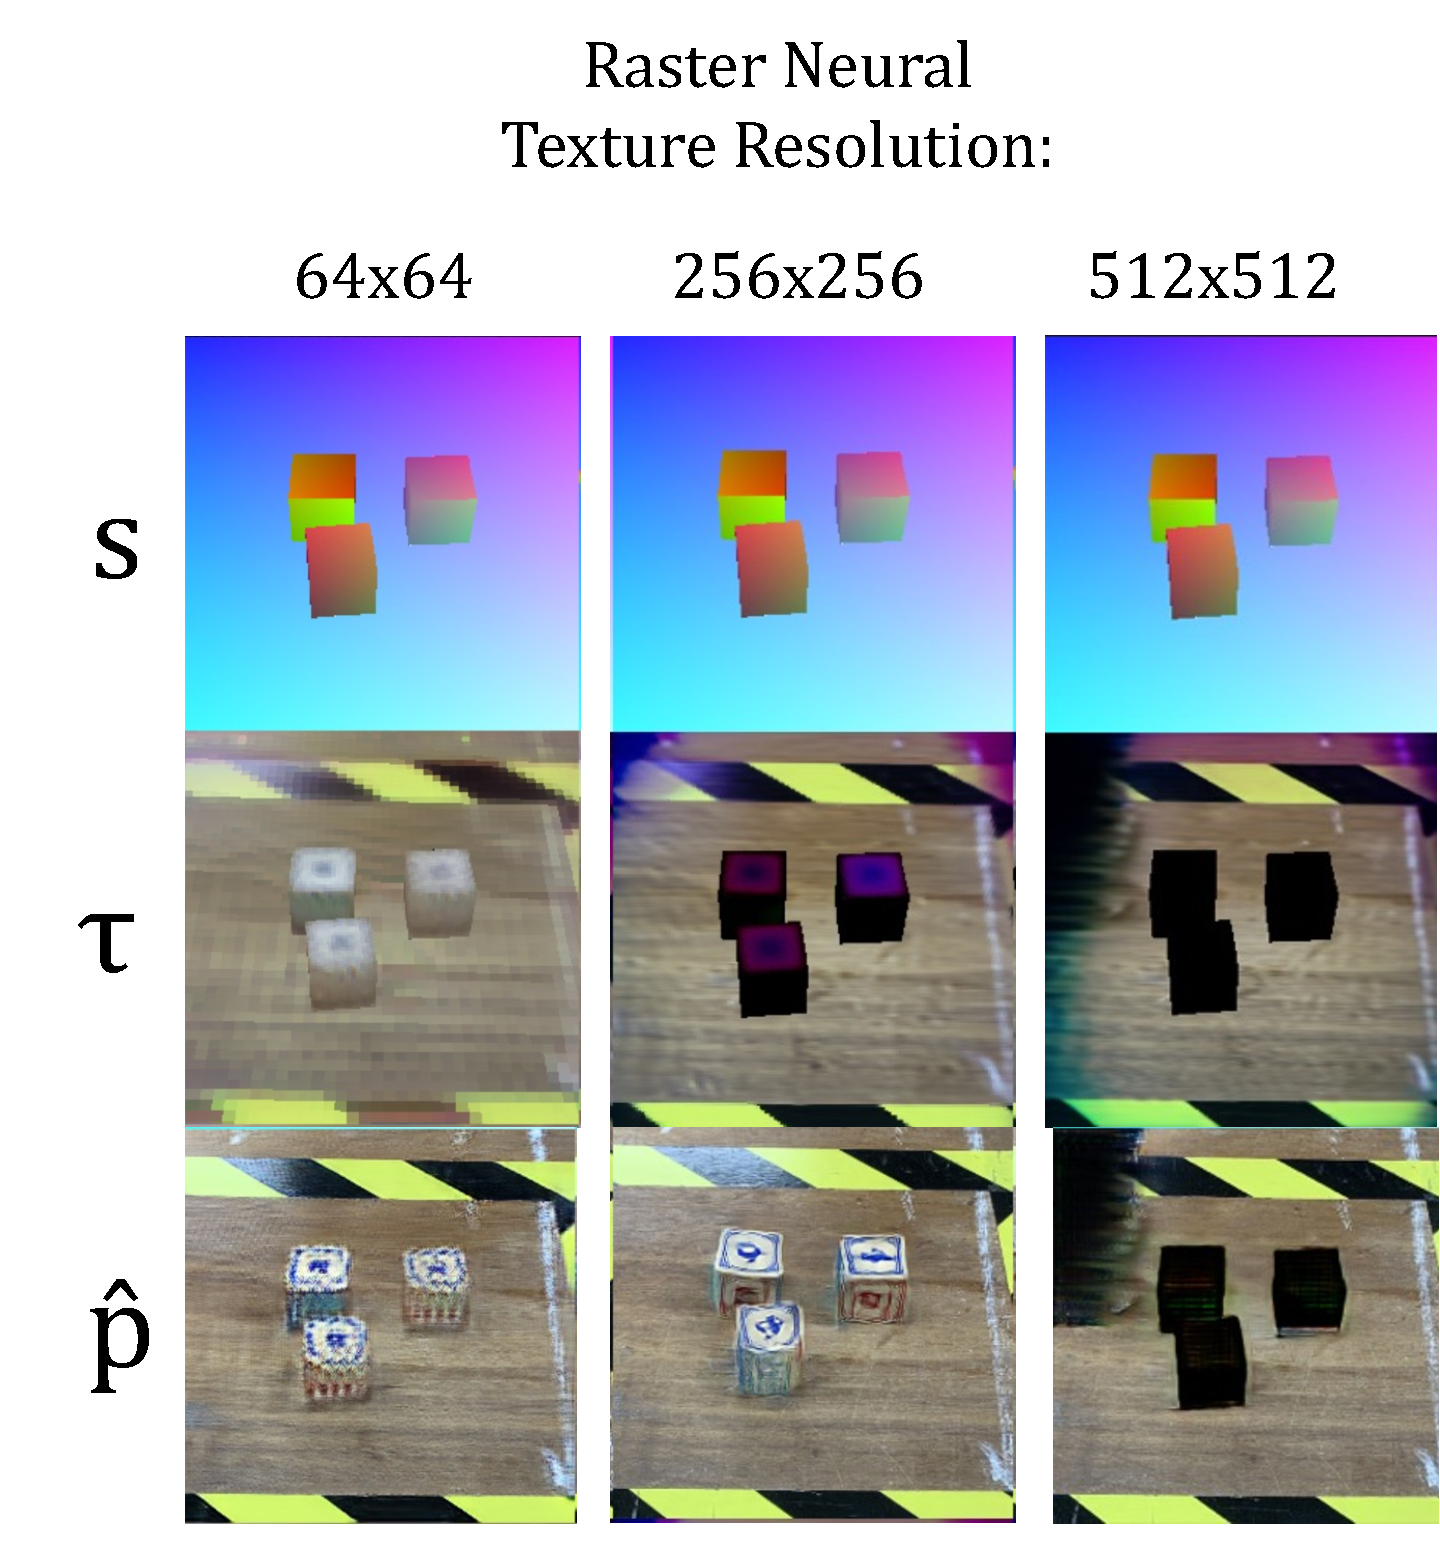
\includegraphics[width=400pt]{../images/raster_texture_resolution_comparisons.pdf}
		\end{center}
		\caption{
			The resolution of the raster neural texture seriously impacts performance in ``Raster TRITON''. Each column has a different neural texture resolution.
			The neural texture only looks like the translation when the resolution is low.
		}
		\label{fig:raster_texture_resolution_comparisons}
	\end{figure}

	In this paragraph we offer possible explanations for these observations.
	With raster-based textures, only the side of an object that currently is seen in a view is allowed to change during each update, because the gradient can't be propagated into pixels that aren't seen.
	If this means changing overall brightness of an object for example, the brightness of that object can't be changed over the entire object until every side has been seen - which won't happen in a single iteration, since the batch size is limited.

	In addition to not propagating the gradient to unseen sides of objects, it also can't propagate to texels in-between the UVL values seen in a scene image.
	When the raster neural texture is too large, aliasing effects occur: if you have a raster texture with very high resolution, the loss gradient is less likely to be passed to a given texel because the chance that a given UV value in a scene will be rounded to that pixel's coordinates is very small.
	In practice, this makes large raster neural textures unstable and limits us to using small amounts of detail.
	With neural neural textures, this aliasing problem is mostly mitigated, because when a certain texture receives a gradient at particular UV coordinates, the areas of the texture between those coordinates are also changed.

\subsection{Unprojection Consistency Loss: More Details}

	Here, we give more details about unprojection consistency loss $\lUC$.

	The exact equation for $\lUC$ is as follows:
	to formally define $\lUC$ we define unprojections $\unprojection^{1...N,1...L}$ and mean unprojections (aka recovered textures) $\bar{\unprojection}^{1...L}$ 
	with each $\unprojection^{n,i}\in\real^{3\times128\times128}$:
	%Jinghyan's Version (uses expectation)
	% \begin{equation}
	% 	\unprojection_{U,V}^{n,i}=\expectation\ph_{x,y}^n 
	% 	\eqand \bar{\unprojection}^i_{u,v}   =   
	% 		\frac{1}{N} \lsum_n\unprojection^{n,i}_{u,v} 
	% 	\eqand 
	% 	%\lUC=\frac{\lsum_{i,U,V}
	% 	%\sqrt[]{\frac{1}{N}\lsum_n\left(\bar{\unprojection}^i_{u,v}-\unprojection^{i,n}_{U,V}\right)^2}}
	% 	%{128\cdot128\cdot L}
	% 	\lUC=\mathbb{E}\left[
	% 	\sqrt[]{\frac{1}{N}\lsum_n\left(\bar{\unprojection}^i_{u,v}-\unprojection^{i,n}_{U,V}\right)^2} \right]
	% \end{equation}
	%
	%
	%Unabbreviated: Not Jinguan's version; 
	\begin{multline}
		\unprojection_{c,U,V}^{n,i}=\expectation\ph_{c,x,y}^n 
		\eqand \bar{\unprojection}^i_{c,u,v}   =   
			\frac{1}{N} \lsum_{n=1}^N\unprojection^{n,i}_{c,u,v} 
		\eqand \\
		\lUC=\frac{\lsum_{i=1}^L\lsum_{c=1}^3\lsum_{U=1}^{128}\lsum_{V=1}^{128}
		\sqrt[]{\frac{1}{N}\lsum_{n=1}^N\left(\bar{\unprojection}^i_{c,u,v}-\unprojection^{i,n}_{c,U,V}\right)^2}}
		{3\cdot128\cdot128\cdot L}
	\end{multline}
	where $U=\lfloor128u\rfloor$ and $V=\lfloor128v\rfloor$ and $i=I(l)$ with
	%  $(u,v,l)=s^n_{1...3,x,y}$
	$u=s^n_{1,x,y}$, $v=s^n_{2,x,y}$, $l=s^n_{3,x,y}$
	for all 
	$n \in \{1...N\}$ , 
	$i \in \{1...L\}$ , 
	$x \in \{1...W\}$ , 
	$y \in \{1...H\}$ , 
	$U \in \{1...128\}$ , 
	$V \in \{1...128\}$.

	\bigskip
	
	The hyperparameter 128 we described in section \ref{sec:unprojection_consistency_loss} refers to the resolution of the unprojections used to calculate $\lUC$.
	In figure \ref{fig:unprojection_resolution_comparison} we see that if we were to set it higher, the gradient wouldn't affect the neural texture as densely.

	\begin{figure}[H]
		\begin{center}
			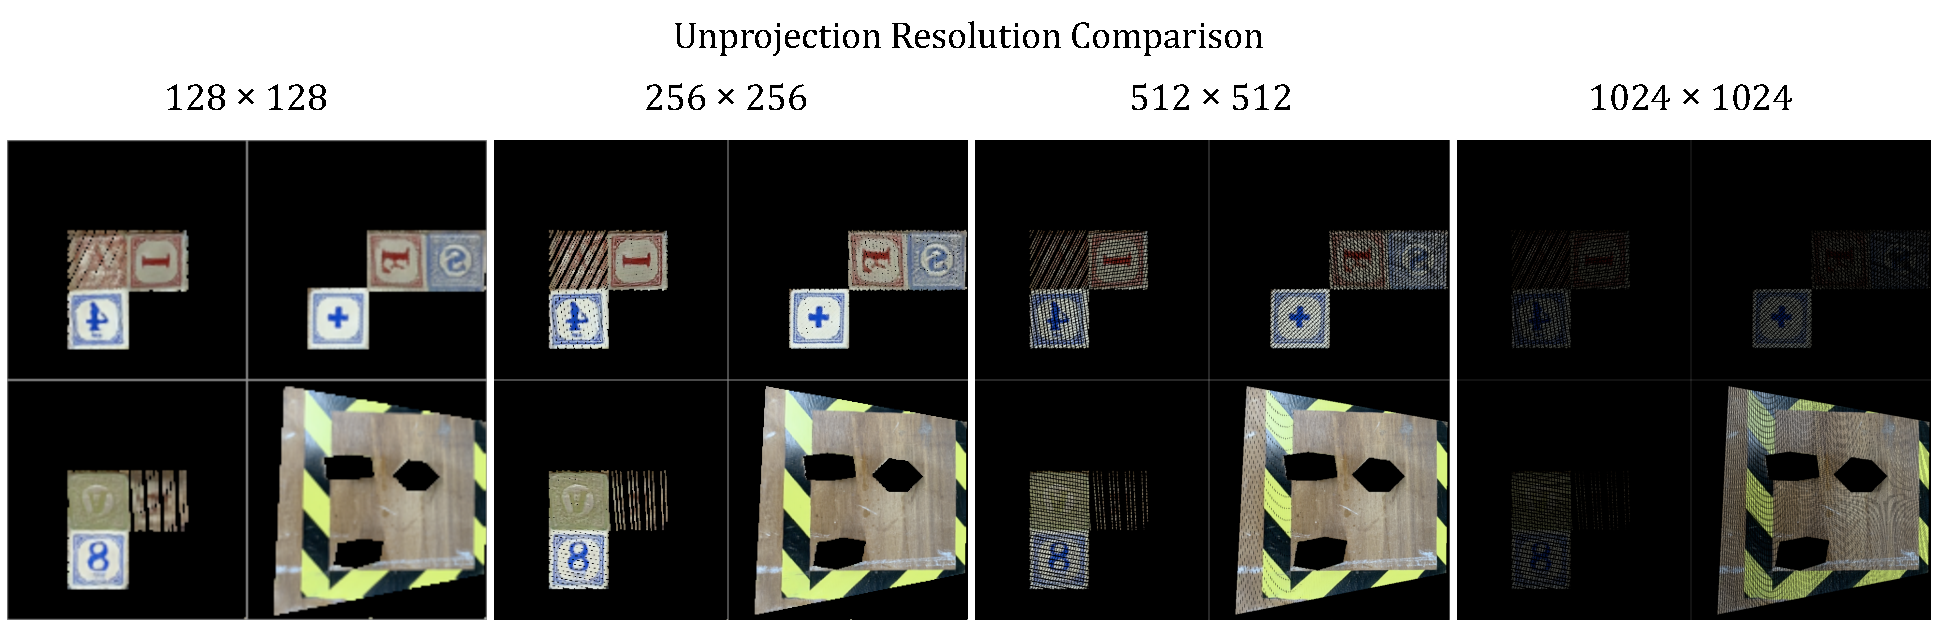
\includegraphics[width=400pt]{../images/unprojection_resolution_comparison.pdf}
		\end{center}
		\caption{
			Here, we unproject a single fake photo $\ph^i$. The resolution of the unprojection matters for unprojection consistency loss. The larger it is, the more precise the alignment will be but the less likely a given UV value is to be assigned a loss greater than 0, creating numerical instability and slowing down learning. 
			When the unprojection resolution is too high, only a few areas of the neural texture will receive a gradient during backpropogation. In practice we use the resolution $128\times128$.
		}
		\label{fig:unprojection_resolution_comparison}
	\end{figure}

\subsection{Training Procedures}

	In this section we detail the training procedures used to create results in section \ref{sec:results} from Triton, CycleGAN, CUT,
		TRITON w/o $\lUC$ (aka TRITON with neither unprojection consistency loss nor texture reality loss), and
		TRITON w/o $\psi, \lUC$ (aka TRITON without textures, and therefore also without unprojection consistency loss or texture reality loss).

	\subsubsection{TRITON}
	\label{par:triton}
	We train TRITON for 200,000 iterations on all datasets. This takes about 36-48 hours on an NVIDIA RTX A5000. 
	The dimension of each input scene is defined by hyperparameter height $H$; the width is scaled to match the aspect ratio of the original input.
	To avoid running out of video memory, we randomly crop each input to a $256\times256$ subset and run TRITON on that cropped input.
	We use batch size 5 during training.
	
	We found that the best way to train TRITON is to start with smaller $H$ values and progressively increase that value during training.
	For the first 50,000 iterations we use $H=320$, then for the next 50,000 iterations $H=420$, then for the last 100,000 iterations $H=\text{(the height of the original input scene)}$.

	\subsubsection{TRITON w/o $\lUC$}
	\label{par:triton_without_luc}
	This ablation is also known as ``Texture-Only'' TRITON, because it has a learnable texture $\psi$ but no consistency losses.
	Its trained the same way that we train TRITON normally as discussed above in \ref{par:triton}, except the surface consistency losses $\lUC$ and $\lTR$ are omitted.
	Effectively, it performs better than MUNIT-like TRITON (aka TRITON w/o $\psi, \lUC$, discussed in \ref{par:munit_triton})
	% It still has a learnable texture $\psi$ though, which is allowed to change however it likes.

	\subsubsection{TRITON w/o $\psi, \lUC$}
	\label{par:munit_triton}
	This ablation is very similar to MUNIT, as TRITON is based on MUNIT and this ablation has neither learnable texture nor consistency losses.
	Like in subsection \ref{par:triton_without_luc}, this ablation shares the same training procedures as TRITON.

	\subsubsection{CycleGAN}
	\label{par:cyclegan}
	We use the original implementation of CycleGAN, and stick to the reccomended 200 epochs, as it tends to overfit if you go further. 
	For our tests, we run CycleGAN on multiple different scales of the input scenes, with input sizes $286\times286$ (CycleGAN's default), $320\times320$, $420\times420$ and $512\times512$. 
	After translation, we stretch the image into the input's aspect ratio.
	We also set $\lambda_{identity}=0$, meaning we disable the identity loss.
	The reported results are the calculated using the best results among these resolutions.
	This dramatically improves CycleGAN's performance when translating UVL scenes to photographs, as this loss was built with the assumption that some parts of the input should not be changed during translation (which is not true in our case).
	
	\subsubsection{CUT}
	\label{par:cut}
	We use the original implementation of CUT, and stick to the recommended 400 epochs, as it tends to overfit if you go further. 
	Like with CycleGAN in \ref{par:cyclegan}, we run CUT on multiple different resolutions of the input scenes, with input sizes $286\times286$ (CUT's default), $320\times320$, $420\times420$ and $512\times512$. 
	After translation, we stretch the image into the input's aspect ratio.
	The reported results are the calculated using the best results among these resolutions.

\subsection{More Results}

	\subsubsection{Unprojection Comparisons}

		In this section we expand on the results in subsection \ref{sec:datasetsresults} by showing the mean unprojection for different image translation algorithms. With the 14 UVL images and corresponding fake photos (or photos) as calculated in \ref{sec:datasetsresults}, we average their unprojections.
		If a translation algorithm is consistent, these unprojections should align well and the average $bar{\omega}$ should not be blurry.

		\begin{figure}[H]
			\begin{center}
				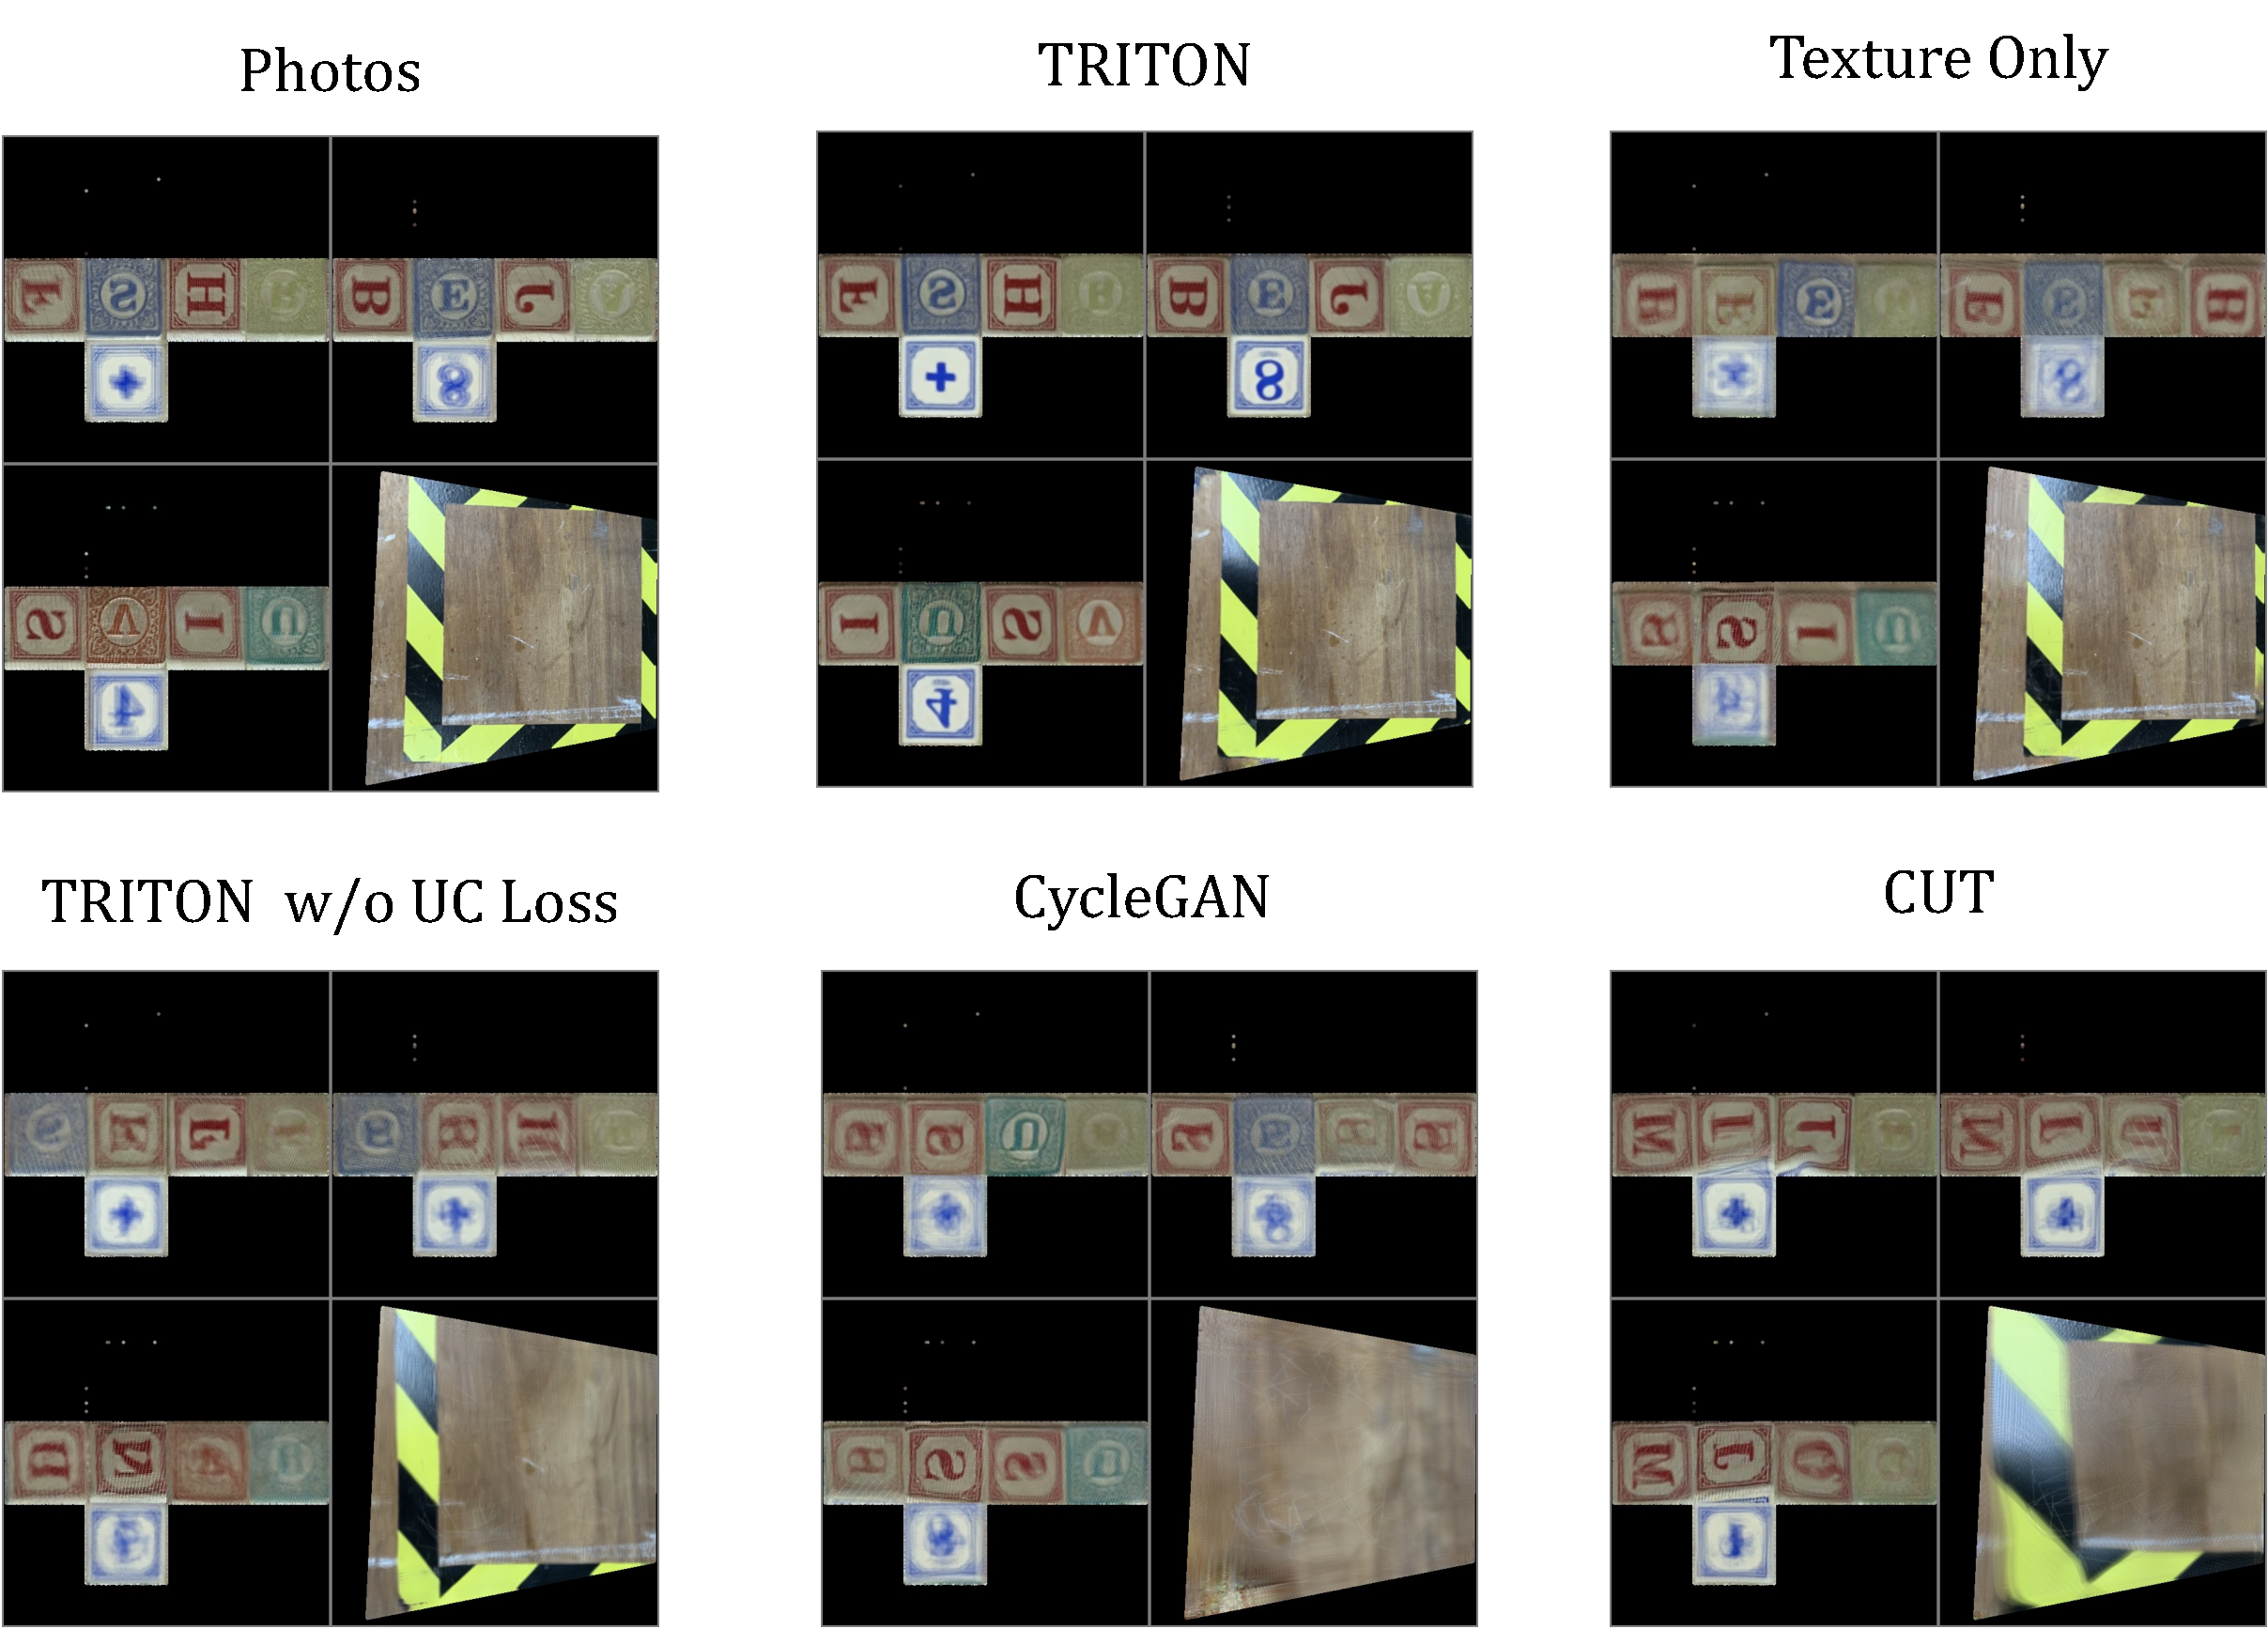
\includegraphics[width=400pt]{../images/unprojection_comparisons.pdf}
			\end{center}
			\caption{
				In this figure, we compare the mean unprojections $\bar{\omega}$ of the 14 labeled images between different algorithms, and compare it to a ground truth. In this diagram, we align all the unprojections to make them easier to compare. Note how TRITON is more crisp and matches the unprojected photographs better than the other algorithms, which are blurrier and have the wrong colors and letters on each side of the alphabet blocks. CycleGAN and CUT for example incorrectly duplicate letters between alphabet blocks.
			}
			\label{fig:unprojection_resolution_comparison}
		\end{figure}


	\subsubsection{Videos}

		We have created animations using TRITON to see how consistency helps:

		https://youtu.be/fuTSta_M6NQ
	
		


	

	





\begin{comment}
\clearpage

\section*{Appendix} 
\label{sec:appendix}

    \subsection{Unsorted}
     	These neural textures are not stored in raster form during training. Instead, as illustrated in figure \ref{fig:learnable_textures}, they're paramaterized by pixel-wise fourier feature networks \cite{fourier_feature_networks} that take in UV coordinates and returns RGB colors. During inference, however, these textures are rasterized to save both time and video memory.

	\subsection*{Unprojection Recovery Resolution Effect}

		Also, the resolution of the unprojection matters:



		\begin{figure}[H]
			\begin{center}
				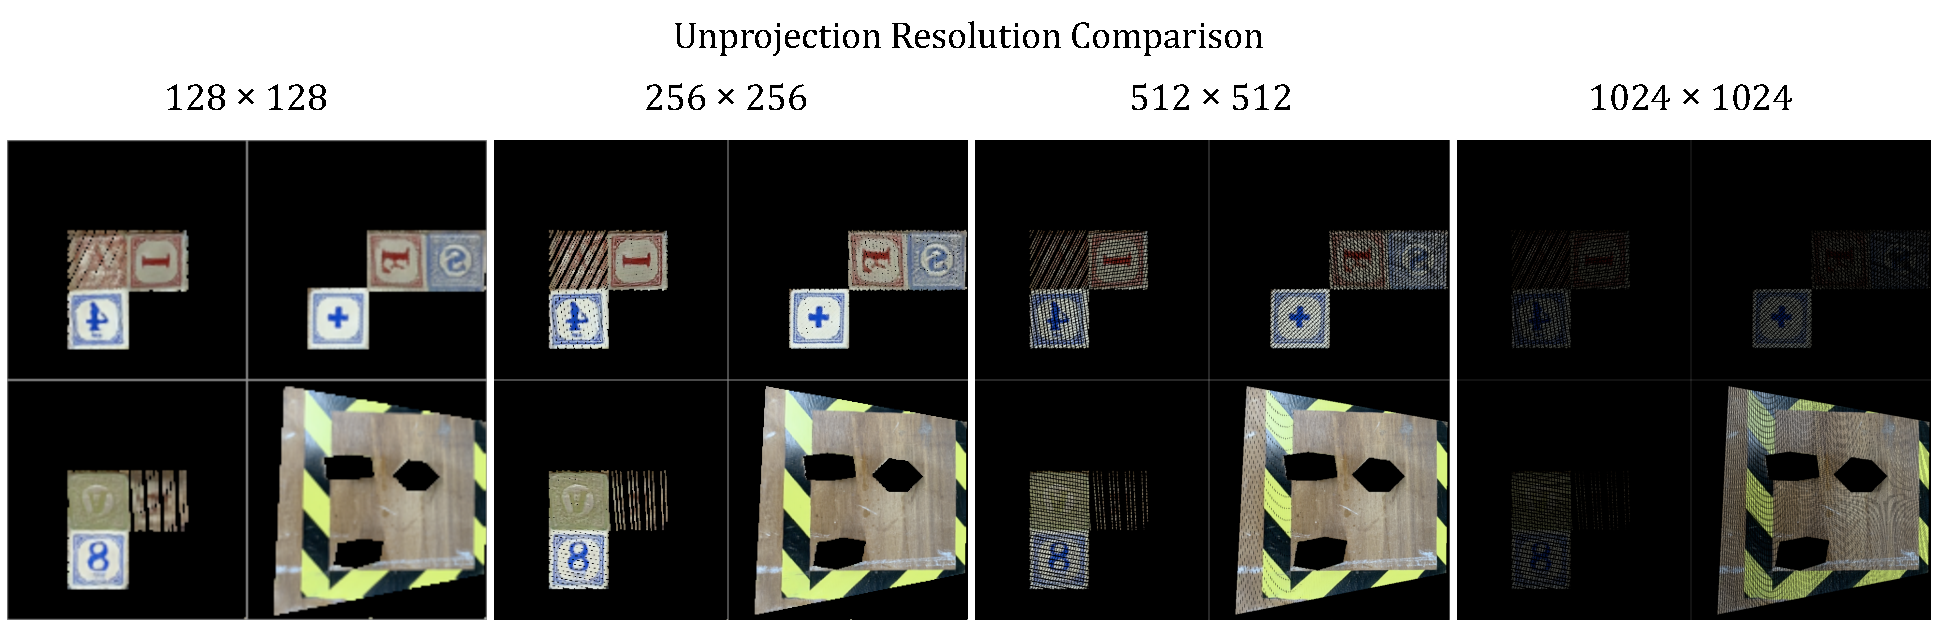
\includegraphics[width=400pt]{../images/unprojection_resolution_comparison.pdf}
			\end{center}
			\caption{
				The resolution of an unprojection matters for unprojection consistency loss. The larger it is, the more precise the alignment will be but the less likely a given UV value is to be assigned a loss greater than 0, lowering numerical instability.
			}
			\label{fig:unprojection_resolution_comparison}
		\end{figure}

	\subsection*{Texture Realism Theory}
		\label{sec:texture_realism_theory}


		THIS SECTION IS UNPOLISHED, BUT CONTAINS  THE NESSECARY CONTENT.
		I'll delete this section if you don't think its important enough to keep.

		Texture realism loss equation:
		$L_{TR}=L_{TR_{l2}}+L_{TR_{msssim}}$
		where 
		$L_{TR_{msssim}} = -msssim(\pi,\hat{p})$ and
		$L_{TR_{l2}} = \frac{
			\lsum_{i=1}^B {
			%  \mu\left(u_{1\dots B,\ 1\dots L}\right)_{1...L}
			\left( \pi-\hat{p}  \right)^2
				} 
		}
		{B}$

		There's a good reason for this: it's almost equivalent to unprojection consistency.
		In fact, it can even be used on its own without unprojection consistency loss (both are sufficient to translate things.)

		(Give theoretical explation)
		$
		\ell_{UC} = 
		\
		\
		\mu\left(\sigma\left(u_{1\dots B,\ 1\dots L}\right)_{1 \dots L}\right) = 
		\sqrt{
		\frac{
			\lsum_{i=1}^B {
				%  \mu\left(u_{1\dots B,\ 1\dots L}\right)_{1...L}
				\left( \hat{p}-\bar{p}  \right)^2
				} 
			}
			{B}
		}
		$
		Using $\bar{p}$ from figure \ref{fig:unprojection_consistency_loss}

		Because $\bar{p}$ is created from the average recovered textures of $\hat{p}$, $\bar{p} \approx \hat{p}$.

		Because of texture realism loss, $\pi \approx \hat{p}$.

		Therefore, $\bar{p} \approx \hat{p} \approx \pi$


		% The l2 component of the texture realism loss equation:
		% $ \
		% \
		% \
		% \
		% \ \ell_{TR_{l2}}=\sum\limits_{i=1}^B {
		% 	%  \mu\left(u_{1\dots B,\ 1\dots L}\right)_{1...L}
		% 	\left( \pi-\hat{p}  \right)^2
		% 	 } 
		% $

		Substituting one projected texture for another, aka $\pi$ for $\bar{p}$, we get 
		$ \
		\
		\
		\
		\ \ell_{TR_{l2}}
		\approx
		\frac{\sum\limits_{i=1}^B {
			%  \mu\left(u_{1\dots B,\ 1\dots L}\right)_{1...L}
			\left( \hat{p}-\pi  \right)^2
			}}{B} = \ell_{UC}^2
		$


		\subsection{Color Loss}

		TRITON is very robust to geometric imperfections. However, sometimes it takes this a bit too far - it can over-fit textures onto the wrong objects and still maintain consistency.
		In one example, it manages to map an apple texture onto a cube. 

		To help TRITON correctly match textures to objects, we introduce a small amount of supervision by adding a color loss. I'm going to stop writing this because I don't know if I even want to keep this in the paper...you can achieve the same result by running the algorithm multiple times, and so its not strictly necessary.

		ASK MICHAEL: I'd rather not mention this entire section and run out the page limit...it's not very important, and not used in the robot experiments. It's only used in the experiment with the five items including the apple. Can we add it to the appendix instead?


\section*{Graveyard}

Here I put things I won't include in the paper or appendix, but want to keep for reference until submission

\begin{figure}[H]
	\begin{center}
		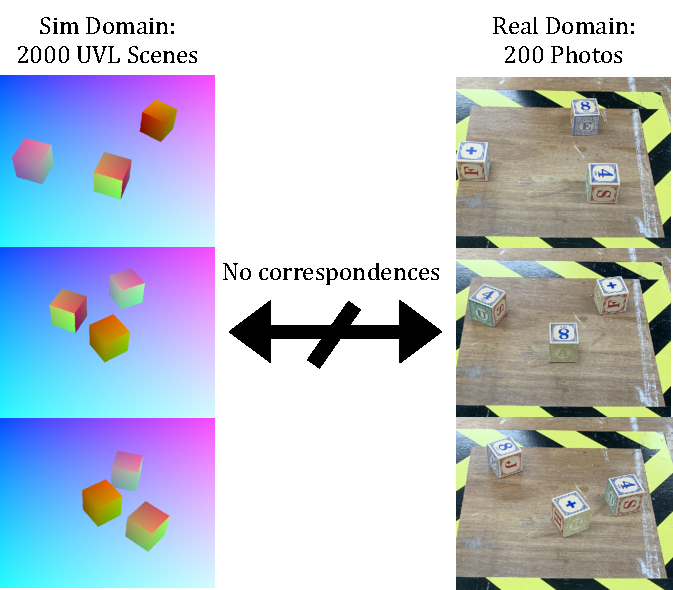
\includegraphics[width=200pt]{../images/dataset_explanation.pdf}
	\end{center}
	\caption{
		Compatible datasets have two sets of images: a set of UVL scenes and a set of photographs.
		TRITON is a sim-to-real image translation algorithm, taking in synthetic UVL scenes and aiming to create realistic fake photographs. 
		Being an unsupervised algorithm, there are no correspondences between synthetic and real images.
		In this dataset, three alphabet cubes are moved around the table. 
		The synthetic and rear cameras have the same position and field of view.
		There are many more UVL scenes than photos because synthetic scenes can be generated automatically whereas photos require real-world labor.
		}
	\label{fig:dataset_explanation}
\end{figure}


\section*{Things to Ask Michael}


QUESTIONS FOR MICHAEL:
\begin{itemize}
	\item - TODO: WE MAINTAIN WHAT WE NOW CALL "SURFACE CONSISTENCY" instead of view consistency! Or texture consistency? Etc? What should we call it?
\end{itemize}

\end{comment}

\end{document}